%%%%%%%%%%%%%%%%%%%%%%%%%%%%%%%%%%%%%%%%%%%%%%%%%%%%%%%%%%%%%%%%%%%%%%%%%%%%%
%%                                                                           
%%   The `compliation' paper for all z>5 spec-z quasars, here called "Very High Redshift Quasars" (VHzQs) and 
%%   looking into their IR properties. Motivations include putting a list of all the VHzQ in one place, looking for 
%%   signs of super-critical accretion and having a super-set of objects and their given parameters ahead of 
%%   JWST GO Cycle 1. 
%%									    
%%%%%%%%%%%%%%%%%%%%%%%%%%%%%%%%%%%%%%%%%%%%%%%%%%%%%%%%%%%%%%%%%%%%%%%%%%%%%
\documentclass[usenatbib]{mnras}

\usepackage{graphicx,fancyhdr,natbib,subfigure}
\usepackage{epsfig, epsf}
\usepackage{amsmath, cancel, amssymb}
\usepackage{lscape, longtable, caption}
\usepackage{multirow}
\usepackage{dcolumn}% Align table columns on decimal point
\usepackage{bm}% bold math
\usepackage{hyperref,ifthen}
\usepackage{verbatim}
\usepackage{color}
\usepackage[usenames,dvipsnames]{xcolor}
%% http://en.wikibooks.org/wiki/LaTeX/Colors



%%%%%%%%%%%%%%%%%%%%%%%%%%%%%%%%%%%%%%%%%%%
%       define Journal abbreviations      %
%%%%%%%%%%%%%%%%%%%%%%%%%%%%%%%%%%%%%%%%%%%
\def\nat{Nat} \def\apjl{ApJ~Lett.} \def\apj{ApJ}
\def\apjs{ApJS} \def\aj{AJ} \def\mnras{MNRAS}
\def\prd{Phys.~Rev.~D} \def\prl{Phys.~Rev.~Lett.}
\def\plb{Phys.~Lett.~B} \def\jhep{JHEP} \def\nar{NewAR}
\def\npbps{NUC.~Phys.~B~Proc.~Suppl.} \def\prep{Phys.~Rep.}
\def\pasp{PASP} \def\aap{Astron.~\&~Astrophys.} \def\araa{ARA\&A}
\def\pasa{PASA}
\def\jcap{\ref@jnl{J. Cosmology Astropart. Phys.}}%
\def\physrep{Phys.~Rep.}


\newcommand{\preep}[1]{{\tt #1} }

%%%%%%%%%%%%%%%%%%%%%%%%%%%%%%%%%%%%%%%%%%%%%%%%%%%%%
%              define symbols                       %
%%%%%%%%%%%%%%%%%%%%%%%%%%%%%%%%%%%%%%%%%%%%%%%%%%%%%
\def \Mpc {~{\rm Mpc} }
\def \Om {\Omega_0}
\def \Omb {\Omega_{\rm b}}
\def \Omcdm {\Omega_{\rm CDM}}
\def \Omlam {\Omega_{\Lambda}}
\def \Omm {\Omega_{\rm m}}
\def \ho {H_0}
\def \qo {q_0}
\def \lo {\lambda_0}
\def \kms {{\rm ~km~s}^{-1}}
\def \kmsmpc {{\rm ~km~s}^{-1}~{\rm Mpc}^{-1}}
\def \hmpc{~\;h^{-1}~{\rm Mpc}} 
\def \hkpc{\;h^{-1}{\rm kpc}} 
\def \hmpcb{h^{-1}{\rm Mpc}}
\def \dif {{\rm d}}
\def \mlim {m_{\rm l}}
\def \bj {b_{\rm J}}
\def \mb {M_{\rm b_{\rm J}}}
\def \mg {M_{\rm g}}
\def \qso {_{\rm QSO}}
\def \lrg {_{\rm LRG}}
\def \gal {_{\rm gal}}
\def \xibar {\bar{\xi}}
\def \xis{\xi(s)}
\def \xisp{\xi(\sigma, \pi)}
\def \Xisig{\Xi(\sigma)}
\def \xir{\xi(r)}
\def \max {_{\rm max}}
\def \gsim { \lower .75ex \hbox{$\sim$} \llap{\raise .27ex \hbox{$>$}} }
\def \lsim { \lower .75ex \hbox{$\sim$} \llap{\raise .27ex \hbox{$<$}} }
\def \deg {^{\circ}}
%\def \sqdeg {\rm deg^{-2}}
\def \deltac {\delta_{\rm c}}
\def \mmin {M_{\rm min}}
\def \mbh  {M_{\rm BH}}
\def \mdh  {M_{\rm DH}}
\def \msun {M_{\odot}}
\def \z {_{\rm z}}
\def \edd {_{\rm Edd}}
\def \lin {_{\rm lin}}
\def \nonlin {_{\rm non-lin}}
\def \wrms {\langle w_{\rm z}^2\rangle^{1/2}}
\def \dc {\delta_{\rm c}}
\def \wp {w_{p}(\sigma)}
\def \PwrSp {\mathcal{P}(k)}
\def \DelSq {$\Delta^{2}(k)$}
\def \WMAP {{\it WMAP \,}}
\def \cobe {{\it COBE }}
\def \COBE {{\it COBE \;}}
\def \HST  {{\it HST \,\,}}
\def \Spitzer  {{\it Spitzer \,}}
\def \ATLAS {VST-AA$\Omega$ {\it ATLAS} }
\def \BEST   {{\tt best} }
\def \TARGET {{\tt target} }
\def \TQSO   {{\tt TARGET\_QSO}}
\def \HIZ    {{\tt TARGET\_HIZ}}
\def \FIRST  {{\tt TARGET\_FIRST}}
\def \zc {z_{\rm c}}
\def \zcz {z_{\rm c,0}}

\newcommand{\ltsim}{\raisebox{-0.6ex}{$\,\stackrel
        {\raisebox{-.2ex}{$\textstyle <$}}{\sim}\,$}}
\newcommand{\gtsim}{\raisebox{-0.6ex}{$\,\stackrel
        {\raisebox{-.2ex}{$\textstyle >$}}{\sim}\,$}}
\newcommand{\simlt}{\raisebox{-0.6ex}{$\,\stackrel
        {\raisebox{-.2ex}{$\textstyle <$}}{\sim}\,$}}
\newcommand{\simgt}{\raisebox{-0.6ex}{$\,\stackrel
        {\raisebox{-.2ex}{$\textstyle >$}}{\sim}\,$}}

\newcommand{\Msun}{M_\odot}
\newcommand{\Lsun}{L_\odot}
\newcommand{\lsun}{L_\odot}
\newcommand{\Mdot}{\dot M}

\newcommand{\sqdeg}{deg$^{-2}$}
\newcommand{\hi}{H\,{\sc i}\ }
\newcommand{\lya}{Ly$\alpha$\ }
%\newcommand{\lya}{Ly\,$\alpha$\ }
\newcommand{\lyaf}{Ly\,$\alpha$\ forest}
%\newcommand{\eg}{e.g.~}
%\newcommand{\etal}{et~al.~}
\newcommand{\lyb}{Ly$\beta$\ }
\newcommand{\cii}{C\,{\sc ii}\ }
\newcommand{\ciii}{C\,{\sc iii}]\ }
\newcommand{\civ}{C\,{\sc iv}\ }
\newcommand{\SiII}{Si\,{\sc ii}\ }
\newcommand{\SiIV}{Si\,{\sc iv}\ }
\newcommand{\mgii}{Mg\,{\sc ii}\ }
\newcommand{\feii}{Fe\,{\sc ii}\ }
\newcommand{\feiii}{Fe\,{\sc iii}\ }
\newcommand{\caii}{Ca\,{\sc ii}\ }
\newcommand{\halpha}{H\,$\alpha$\ }
\newcommand{\hbeta}{H\,$\beta$\ }
\newcommand{\hgamma}{H\,$\gamma$\ }
\newcommand{\hdelta}{H\,$\delta$\ }
\newcommand{\oi}{[O\,{\sc i}]\ }
\newcommand{\oii}{[O\,{\sc ii}]\ }
\newcommand{\oiii}{[O\,{\sc iii}]\ }
\newcommand{\heii}{He\,{\sc ii}\ }
%\newcommand{\heii}{[He\,{\sc ii}]\ }
\newcommand{\nv}{N\,{\sc v}\ }
\newcommand{\nev}{Ne\,{\sc v}\ }
\newcommand{\neiii}{[Ne\,{\sc iii}]\ }
\newcommand{\alii}{Al\,{\sc ii}\ }
\newcommand{\aliii}{Al\,{\sc iii}\ }
\newcommand{\siiii}{Si\,{\sc iii}]\ }


\begin{document}

\title[Very high-$z$ Quasars]
        {Near and Mid-infrared properties of known $z\geq5$ Quasars}
\author[Ross \& Cross]
       {Nicholas P. Ross$^{1}$\thanks{Corresponding Author: npross@roe.ac.uk} and Nicholas J. G. Cross$^{1}$
\\ 
$^1$Institute for Astronomy, University of Edinburgh, Royal Observatory, Edinburgh, EH9 3HJ, United Kingdom\\
}

\maketitle
\begin{abstract}
%For the first time since the discovery of $z\geq5.00$ quasars, 
%In this paper, 
We assemble a catalogue of 463 
spectroscopically confirmed very high ($z\geq5.00$) redshift 
quasars %in one catalogue.  
%In particular we present the near
and report their near ($zZyYJHK_{s}$ and $K$) infrared and mid-infrared (WISE) properties. 
%of all 463 spectroscopically confirmed redshift $z\geq5.00$ quasars.
Using archival WFCAM/UKIRT and VIRCAM/VISTA data we check for
photometric variability in the near-infrared that might be expected
from super-Eddington accretion and find {\it blah}.  
%%
% We present a comprehensive series of colour-redshift and colour-colour plots and make inferences into the hot dust properties of the very high-redshift quasar population. aq
Extrapolating the known quasar luminosity function
we suggest that $x$\% of the possibly detected $z\geq5$ quasars in the
current datasets have been discovered. 
All the data, analysis codes and plots used and generated here can be found at:
\href{https://github.com/d80b2t/VHzQ}{\tt github.com/d80b2t/VHzQ}.
\end{abstract}


\begin{keywords}
Astronomical data bases: surveys -- 
Quasars: general -- 
galaxies: evolution -- 
galaxies: infrared.
\end{keywords}



%%%%%%%%%%%%%%%%%%%%%%%%%%%%%%%%%%%%%%%%%%%%%%%%%%%%%%%%%%%%%%%%%%
%%%%%%%%%%%%%%%%%%%%%%%%%%%%%%%%%%%%%%%%%%%%%%%%%%%%%%%%%%%%%%%%%%
%%
%%  S E C T I O  N   1         S E C T I O  N   1           S E C T I O  N   1       S E C T I O  N   1
%%  S E C T I O  N   1         S E C T I O  N   1           S E C T I O  N   1       S E C T I O  N   1
%%  S E C T I O  N   1         S E C T I O  N   1           S E C T I O  N   1       S E C T I O  N   1
%%
%%%%%%%%%%%%%%%%%%%%%%%%%%%%%%%%%%%%%%%%%%%%%%%%%%%%%%%%%%%%%%%%%%
%%%%%%%%%%%%%%%%%%%%%%%%%%%%%%%%%%%%%%%%%%%%%%%%%%%%%%%%%%%%%%%%%%
\section{Introduction}
Very high redshift quasars (VH$z$Q; defined here to have redshifts $z\geq5.00$) are excellent probes of the early Universe. This includes studies of the Epoch of Reionization for hydrogen \citep[see e.g.][for reviews]{Fan2006review, Mortlock2016}, the formation and build-up of supermassive black holes \citep[e.g., ][]{Rees1984, WyitheLoeb2003, Volonteri2010, Agarwal2016, Valiante2018, Latif2018, Wise2019} and early metal enrichment \citep[see e.g., ][]{Simcoe2012, Chen2017, Bosman2017}.

Super-critical accretion, where $\dot{M} > \dot{M}_{\rm Edd}$, is a viable mechanism to explain the high, potentially super-Eddington, luminosity and rapid growth of supermassive black holes in the early universe \citep[e.g.,][]{AlexanderNatarajan2014, MadauHaardtDotti2014, Volonteri2015, Pezzulli2016, Lupi2016, Pezzulli2017, Takeo2018}. Thus, one could expect VH$z$Qs to potentially vary in luminosity as they go through phases of super-critical accretion. These signatures of photometric variability should be looked for, noting the rest-frame optical emission is redshifted into the observed near-infrared (NIR) at redshifts $z>5$. Fortunately, data are now in place from deep, wide-field NIR instruments and surveys such as the Wide Field Camera (WFCAM) instrument on the United Kingdom Infra-Red Telescope (UKIRT) in the Northern Hemisphere and the VISTA InfraRed CAMera (VIRCAM) on the Visible and Infrared Survey Telescope for Astronomy (VISTA) in the Southern Hemisphere, that are necessary for identifying VH$z$Qs.

Quasars are known to be prodigious emitters of infrared emission, thought to be from the thermal emission of dust grains heated by continuum emission from the accretion disc \citep[e.g.,][]{Richards2006b, Leipski2014, Hill2014, Hickox2017}. Observations in the mid-infrared, e.g. $\sim$3-30$\mu$m allow discrimination between AGN\footnote{Historically, ``quasars'' and ``Active Galactic Nuclei (AGN)'' have described different
luminosity/classes of objects. In recognition of the fact that both terms describe accreting supermassive black holes, we use these terms interchangeably, with a preference for quasar, since we are generally in the higher-$L$ regime \citep[e.g.][]{Haardt2016book}.}  and passive galaxies due to the 1.6$\mu$m ``bump'' entering the MIR at $z\approx0.8-0.9$ \citep[e.g., ][]{Wright1994, Sawicki2002, Lacy2004, Stern2005, Richards2006b, Timlin2016} as well as between AGN and star-forming galaxies due to the presence of Polycyclic Aromatic Hydrocarbon (PAHs) at $\lambda
>3\mu$m \citep[e.g., ][]{Yan2007, Tielens2008}. 

\citet{Jiang2006dust} and \citet{Jiang2010} report on the discovery of a quasar without hot-dust emission in a sample of 21 $z\approx6$ quasars. Such apparently hot-dust-free quasars have no counterparts at low redshift. Moreover, those authors demonstrate that the hot-dust abundance in the 21 quasars builds up in tandem with the growth of the central black hole. But understanding how dust first forms and appears in the central engine remains an open question \citep{WangR2008, WangR2011}.

WISE mapped the sky in 4 passbands, in bands centered at wavelengths of 3.4, 4.6, 12, and 23$\mu$m. The all sky `ALLWISE' catalogue release, contains nearly 750 million detections at high-significance\footnote{\href{wise2.ipac.caltech.edu/docs/release/allwise/expsup/sec2\_1.html}{wise2.ipac.caltech.edu/docs/release/allwise/expsup/sec2\_1.html}}, of which over 4.5M AGN candidates have been identified with 90\% reliability \citep{Assef2018}.  \citet{Blain2013} presented WISE mid-infrared (MIR) detections of 17 (55\%) of the then known 31 quasars at $z > 6$. However, \citet{Blain2013} was compiled with the WISE `All-Sky' data release, as opposed to the superior AllWISE catalogues. That sample only examined the 31 known $z>6$ quasars; our sample has 170 objects with redshift $z \geq 6.00$ (with $x$ detected in WISE {\bf NPR to double check!!}). \citet{Banados2016} reports WISE W1, W2, W3 and W4 magnitudes for the Panoramic Survey Telescope and Rapid Response System 1 \citep[Pan-STARRS1, PS1;][]{Kaiser2002, Kaiser2010}, but with no further investigation into the reddest WISE waveband for the VH$z$Qs.

Critically, we now have available to us new W1 and W2 photometry from the `unWISE Source Catalog' \citep[][]{Schlafly_Meisner2018}, a WISE-selected catalogue that is based on significantly deeper imaging and has a more extensive modeling of crowded regions than the ALLWISE release. For the first time in a catalogue, unWISE takes advantage of the ongoing mid-IR Near-Earth Object Wide-Field Infrared Survey Explorer Reactivation mission \citep[NEOWISE-R; ][]{Mainzer2014}, and achieves depths $\sim$0.7 mag deeper than ALLWISE (in W1/2).  This additional depth is a significant advantage in the detection and study of VH$z$Qs in the 3-5 micron regime.

Here we present for the first time the combined near-infrared properites (from UKIRT and VIRCAM) and the new mid-infrared unWISE for all the spectroscopically known $z\geq5.00$ quasars. Our motivations are numerous and include: {\it (i)} establishing the first complete catalogue of $z>5.00$ quasars since the pioneering work from SDSS; {\it (ii)} utilizing all the WFCAM and VISTA near-infrared photometry available for the quasars; {\it (iii)} making the first study of near- and mid-IR variability of the VHzQ population and {\it (iv)} establishing the photometric properties for upcoming surveys and telescopes including the Large Synoptic Survey Telescope (LSST)\footnote{\href{https://www.lsst.org}{{lsst.org}}}, ESA {\it Euclid}\footnote{\href{https://sci.esa.int/euclid/}{sci.esa.int/euclid/}} and the {\it James Webb Space Telescope} (JWST)\footnote{\href{https://www.jwst.nasa.gov/}{jwst.nasa.gov};}$^,$\footnote{\href{https://sci.esa.int/jwst/}{sci.esa.int/jwst};}$^,$\footnote{\href{https://www.asc-csa.gc.ca/eng/satellites/jwst/}{www.asc-csa.gc.ca/eng/satellites/jwst};}$^,$\footnote{\href{https://jwst.stsci.edu/}{jwst.stsci.edu}}. We chose redshift $z=5.00$ as our lower redshift limit due to a combination of garnishing a large sample, adequately spanning physical properties (e.g. luminosity, age of the Universe) and to highlight the parts of $L-z$ parameter space where $z>5$ quasars still wait to be discovered. 

This paper is organized as follows.  In Section 2, we present the assembled list of the 463 $z\geq5.00$ VH$z$Qs that we have compiled. We then give a high-level overview of the photometric surveys and datasets we use and present the photometry of the VH$z$Qs. In Section 3 we ... and In Section 4 we ... We conclude in Section 5 and present all the necessary details to obtain our dataset in the Appendices. 

We present all our photometry and magnitudes on the AB zero-point system \citep{Oke_Gunn1983, Fukugita1996}.  This includes the near-infrared, as well as the mid-infrared magnitudes. Appendix~\ref{sec:filters} gives the AB to Vega transforms for a wide range of optical, NIR and MIR filters. We use a flat $\Lambda$CDM cosmology with $H0 = 67.7$ km s$-1$ Mpc$−1$, $\Omega_{\rm M} = 0.307$, and $\Omega_{\Lambda} = 0.693$ (Planck Collaboration et al. 2016) to be consistent with \citet{Banados2016} and all logarithms are to the base 10. 




%%%%%%%%%%%%%%%%%%%%%%%%%%%%%%%%%%%%%%%%%%%%%%%%%%%%%%%%%%%%%%%%%%
%%%%%%%%%%%%%%%%%%%%%%%%%%%%%%%%%%%%%%%%%%%%%%%%%%%%%%%%%%%%%%%%%%
%%
%%    S E C T I O  N   2         S E C T I O  N   2           S E C T I O  N   2       S E C T I O  N   2
%%    S E C T I O  N   2         S E C T I O  N   2           S E C T I O  N   2       S E C T I O  N   2
%%    S E C T I O  N   2         S E C T I O  N   2           S E C T I O  N   2       S E C T I O  N   2
%%
%%%%%%%%%%%%%%%%%%%%%%%%%%%%%%%%%%%%%%%%%%%%%%%%%%%%%%%%%%%%%%%%%%
%%%%%%%%%%%%%%%%%%%%%%%%%%%%%%%%%%%%%%%%%%%%%%%%%%%%%%%%%%%%%%%%%%
\begin{figure}
%%trim=l b r t
%  \includegraphics[width=18.6cm, clip,trim=14mm 4mm 10mm 10mm]
  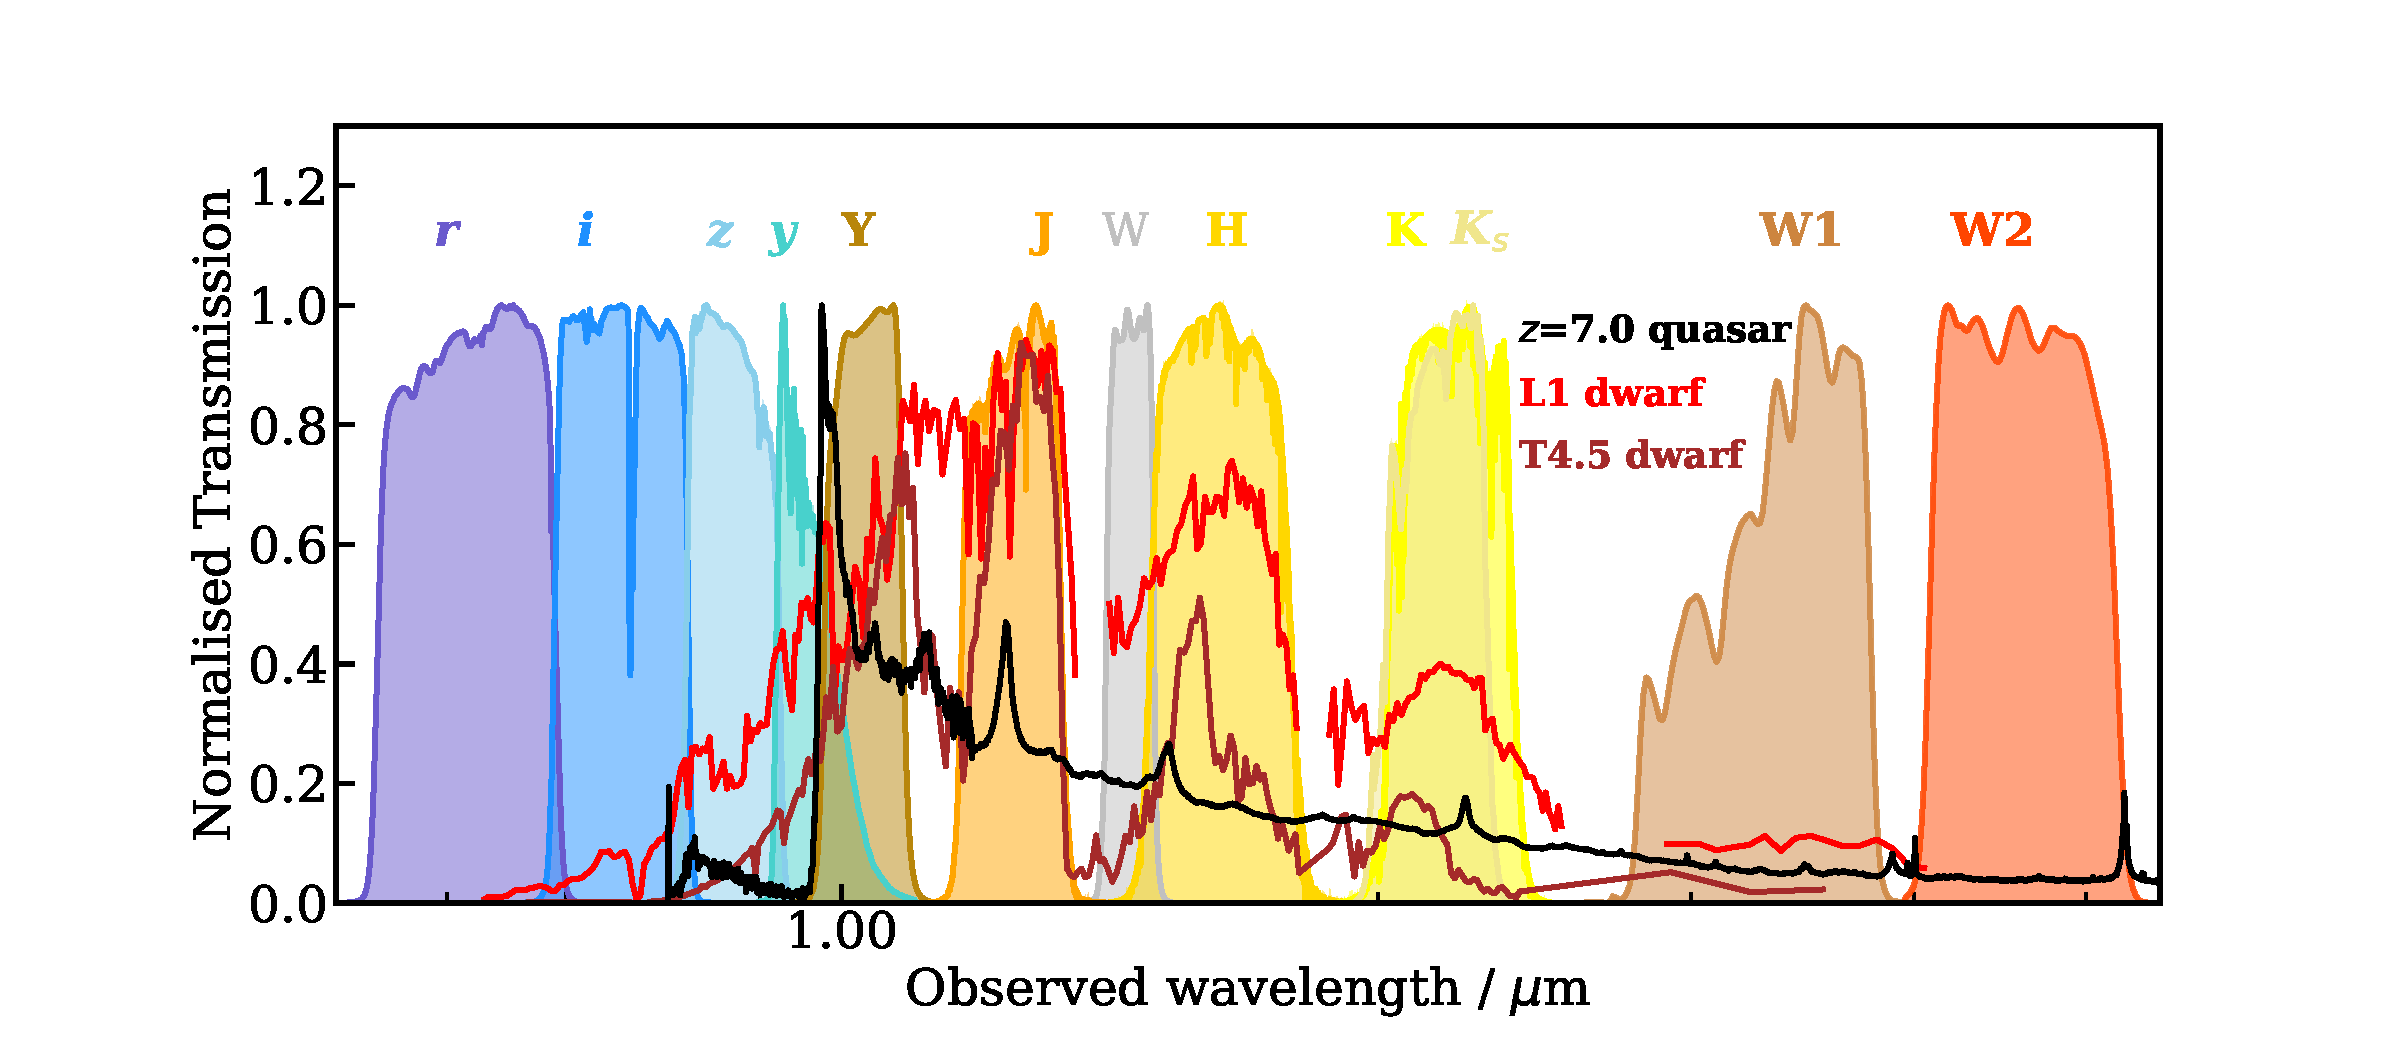
\includegraphics[width=8.6cm, clip,trim=32mm 4mm 32mm 10mm]
  {/cos_pc19a_npr/programs/quasars/highest_z/SEDs/filters_vs_QSOstars_z7pnt0.pdf}
  \centering
  \vspace{-12pt}
  \caption[]
  {The spectral bands used by different survey telescopes and that are relevant here.
    The $grizy$ filters are from the Pan-STARRS survey. The $JHK$ are from 
    UKIRT/WFCAM, while $K_{s}$ is a VISTA/VIRCAM filter. The 
    The narrow W-band centered at $\lambda\approx14,500$\AA\ is a CFHT/Wircam filter. 
    [NJC: Do we use the W-band anywhere?]
    The WISE passbands  W1-4 are also presented.
    The quasar spectrum is a composite based on \citet{VdB2001} and 
    \citet{Banados2016}. The L and T dwarf spectra are from \citet{Cushing2006}. 
  }
  \label{fig:filters}
\end{figure}

\vspace{-16pt}
\section{Method and Data}
Quasars are generally identified by photometric selection followed by spectroscopic confirmation. Here, we reverse this method obtaining first a list of spectroscopic quasars and then obtain photometric information.

We have compiled a list of 463 quasars with redshifts $z\geq5.00$. We use all the $z\geq5.00$ quasars that have been discovered, spectroscopically confirmed and published as of 2018 December 31 (MJD 58483). We then obtain optical, near-infrared and mid-infrared photometry for the spectral dataset. The optical data comes from the Panoramic Survey Telescope and Rapid Response System (Pan-STARRS) survey \citep{Chambers2016}. The near-infrared data comes from two sources: first, the WFCAM \citep[][]{Casali2007} on the UKIRT, primarly, but not exclusively, as part of the UKIRT Infrared Deep Sky Survey \citep[UKIDSS; ][]{Lawrence2007}.  And second, data from the VIRCAM on the VISTA \citep[][]{Emerson2006, Dalton2006}. The mid-infrared, $\lambda=3-30\mu$m wavelength data is from the the Wide-Field Infrared Survey Explorer \citep[WISE;][]{Wright2010, Cutri2013} mission. For reference, Figure~\ref{fig:filters} displays the wavelength and normalised transmission of the filters in question. 

\subsection{Spectroscopy} 
We compile the list of all known, spectroscopically confirmed
quasars from the literature.  This list was complied from a range of
surveys and papers.  Specifically, we use data from:
\citet{Banados2014, Banados2016, Banados2018}, 
\citet{Becker2015}, 
\citet{Calura2014}, 
\citet{Carilli2007, Carilli2010}, 
\citet{Carnall2015}, 
\citet{Cool2006}, 
\citet{DeRosa2011}, 
\citet{Fan2000, Fan2001c, Fan2003, Fan2004, Fan2006, Fan2018}, 
\citet{Goto2006}, 
\citet{Ikeda2017}, 
\citet{Jiang2008, Jiang2009, Jiang2015, Jiang2016},   
\citet{Kashikawa2015}, 
\citet{Koptelova2017}, 
\citet{Kim2015, Kim2018},  
\citet{Kurk2007, Kurk2009}, 
\citet{Leipski2014}, 
\citet{Mahabal2005}, 
\citet{Matsuoka2016,  Matsuoka2018a, Matsuoka2018b},   
\citet{Mazzucchelli2017}, 
\citet{Morganson2012}, 
\citet{Mortlock2009, Mortlock2011},
\citet{McGreer2006, McGreer2013},  
\citet{Reed2015, Reed2017}, 
\citet{Stern2007},  
\citet{Tang2017}, 
\citet{Venemans2007, Venemans2012, Venemans2013, Venemans2015a, Venemans2015b, Venemans2016},
\citet{WangF2016, WangF2017, WangF2018a, WangF2018b},
\citet{Willott2007, Willott2009, Willott2010a, Willott2013b, Willott2015}, 
\citet{Wu2015} 
\citet{YangJ2018a, YangJ2018b}  
and 
\citet{Zeimann2011}. 
%We have obtained a list of 463 spectroscopically confirmed quasars with redshifts $z\geq5.00$. 

Most of these objects are easily identified by their broad Ly$\alpha$ emission line, \nv emission and characteristic shape blueward of 1215\AA\ in the rest-frame. As we shall see, some of the recently discovered objects are close to the galaxy luminosity function characteristic luminosity $M^{*}$, and some have relatively weak or maybe even completely absorbed Ly$\alpha$ \citep[e.g. Figures 7 and 10 in][]{Banados2016}. We leave aside detailed investigation and discussion into spectral features and line strengths, and take as given the published spectra and redshift identifications.

The breakdown of how many VH$z$Q each survey reports is given in Table~\ref{tab:surveys}. The Sloan Digital Sky Survey (SDSS) and the Pan-STARRS1 (PS1; PSO in Table~\ref{tab:surveys}) survey and alone identified over half (54.6\%) of the VH$z$Q population. Data from the Hyper Suprime-Cam (HSC) on the Subaru telecope is responsible for 13.6\% of our dataset (HSC+SHELLQs in Table~\ref{tab:surveys}). The combination of surveys is also vital for identifying VH$z$Qs. The UKIDSS Large Area Survey (ULAS) on its own, or in combination with other surveys is responsible for 6.5\% of the sample (SUV+ULAS) including the highest-$z$ object. Where more than one survey is used for the high-redshift identification (e.g. via shorter-band veto and longer wavelength detection) we follow the discovery paper naming convention.


\begin{table}
\begin{tabular}{l r r l}
\hline  \hline
Survey              & \# VH$z$Qs & (\%) & Survey reference  \\
\hline  
  ATLAS             &     4    &   ( 0.86)    &  \citet{Shanks2015} \\
  CFHQS            &   20    &   ( 4.32)    &  \citet{Willott2007} \\
  DELS               &   16    &   ( 3.46)    &  \citet{Dey2018} \\
  ELAIS              &     1    &   ( 0.22)    &  \citet{Vaisanen2000} \\
  FIRST              &     1    &   ( 0.22)    &  \citet{Becker1995} \\
  HSC                 &    8    &   ( 1.73)    & \citet{Miyazaki2018} \\
  IMS                 &     5    &   ( 1.08)     &  \citet{Kim2015} \\
  MMT               &   12    &   ( 2.59)     &  \citet{McGreer2013} \\
  NDWFS           &     1    &   ( 0.22)    &  \citet{JD1999} \\
  PSO                 &   83   &   (17.93)   &   \citet{Kaiser2002, Kaiser2010} \\
  RD                   &     1   &   ( 0.22)    &  \citet{Mahabal2005} \\
  SDSS                &  170  &    (36.72)    & \citet{EDR} \\
 SDWISE$^{b}$    &   27    &  ( 5.83)    &   \citet{WangF2016} \\
%% SHELLQs    &  $^{c}$63  &  (13.6)   &  \citet{Matsuoka2016} \\  %% if you include 8 objects from the first HSC paper...
  SHELLQs         &    55    &   (11.88)  &  \citet{Matsuoka2016}     \\  
  SUV$^{c}$       &   20     &    ( 4.32)  & \citet{YangJ2017} \\
  UHS               &    1      &  ( 0.22)     &  \citet{WangF2017} \\
  ULAS               &   10   &   ( 2.16)     & \citet{Lawrence2007} \\
  VDES$^{d}$       &   17  &    ( 3.67)     &  \citet{Reed2017} \\
  VHS                 &     1  &     ( 0.22)    & \citet{WangF2018b} \\
  VIK                 &     9    &  ( 1.94)    &  \citet{Edge2013} \\
  VIMOS           &    1      &  ( 0.22)     &   \citet{LeFevre2003} \\
\hline  \hline
\end{tabular}
\caption{The source and number of the VH$z$Q, with the key survey reference also given. 
  Recent survey name and acronyms include: 
  $^{a}$DESI Legacy Imaging Survey; 
  $^{b}$SDWISE = SDSS+WISE; 
  $^{a}$SUV  = SDSS-ULAS/VHS; 
  $^{c}$VDES = VHS/VIKING+DES; 
%  $^{c}$Includes 8 objects with a HyperSuprimeCam \citep[HSC; ][]{Miyazaki2018} designation.
}
      \label{tab:surveys}
\end{table}

\begin{figure}
%%trim=l b r t
  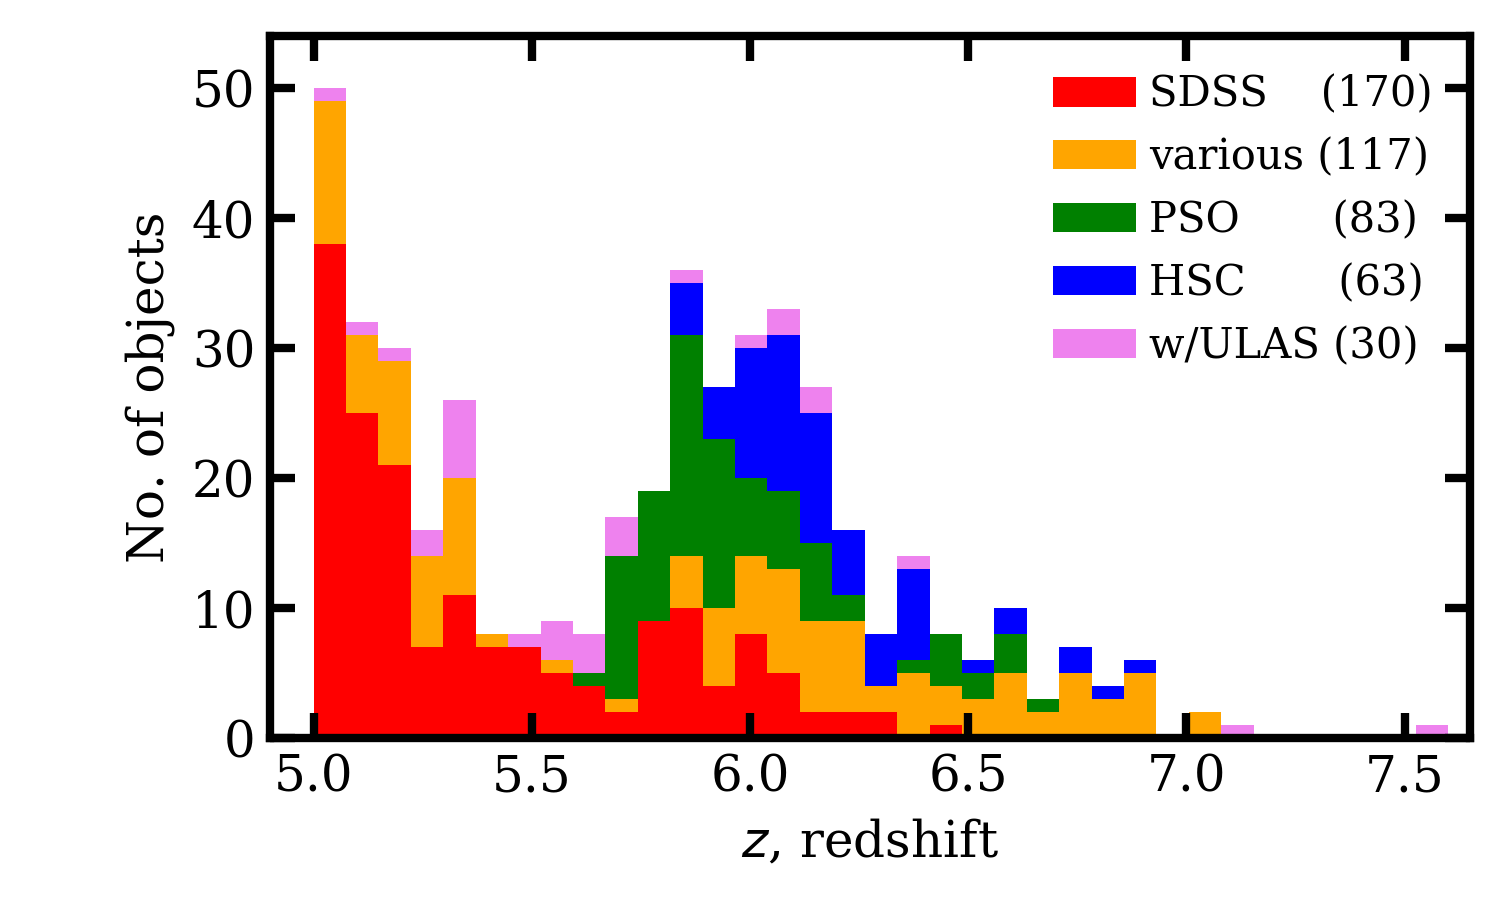
\includegraphics[width=8.0cm, clip, trim=10mm 0mm 0mm 0mm]
  {/cos_pc19a_npr/programs/quasars/highest_z/Nofz/Nofz_0pnt075bins_20181211.png}
  \centering
  \vspace{-12pt}
  \caption[]
  {The redshift distribution $N(z)$ of the VH$z$Q sample. 
    The bins are $\delta-z=0.075$ in width. }
  \label{fig:Nofz}
\end{figure}

The redshifts for the VH$z$Qs generally come from the measurement of
broad UV/optical emission lines. There are far infra-red emission
lines e.g. \cii~158 micron available for several objects, but at the
level of our current analysis broadline redshifts are sufficient.

\begin{table}
\centering
\begin{tabular}{l r  r}
\hline \hline
$z \geq$  & Age / Myr & No. of objects \\
\hline 
7.50         &    700         &   1   \\
7.00         &    767         &   4   \\
6.78         &    800         &  14   \\
6.50         &    845         &  40   \\
6.19         &   900          &  86   \\
6.00         &   937          &  170   \\
5.70         & 1000          &  267   \\
5.00         & 1180          &  463   \\
\hline \hline
\end{tabular}
\caption{The number of objects at or above a given redshift. 
The age of the Universe in megayears is also given. }
      \label{tab:ages}
\end{table}

The number of objects at or above various redshifts, along with the 
corresponding age of the Universe is given in Table~\ref{tab:ages}. 

The $N(z)$ redshift histogram is given for the sample in Figure~\ref{fig:Nofz}. 
We split the contribution up by survey. For clarity we show the individual 
surveys of SDSS, PS1, HSC, the ULAS detection, and tally the remaining 
surveys together (``various''). In Section~\ref{sec:Lz} we discuss the form 
of the $N(z)$ as well as the coverage of the luminosity-redshift $L-z$ plane. 

        
\subsection{Optical Photometry}
We query the Panoramic Survey Telescope and Rapid Response System (Pan-STARRS)\footnote{\href{https://outerspace.stsci.edu/display/PANSTARRS}{https://outerspace.stsci.edu/display/PANSTARRS}} Data Release 1 (DR1) Catalog Archive Server Jobs System (CasJobs) service at \href{http://mastweb.stsci.edu/ps1casjobs/}{mastweb.stsci.edu/ps1casjobs/}. The Pan-STARRS1 (PS1) survey observed the 30,000 deg$^{2}$ of sky north of declination $\delta = -30$ degrees in the five $grizy$ filters. PS1 is the first part of Pan-STARRS to be completed and is the basis for the DR1. \citet{Chambers2016}, \citet{Magnier2016a}, \citet{Waters2016}, \citet{Magnier2016b}, \citet{Magnier2016c} and \citet{Flewelling2016} describe the instrument, survey, and data analyses. The principal science product of the PS1 survey is the catalog accessible through the CasJobs interface.

The PS1 Casjobs SQL Server is located at
\href{http://mastweb.stsci.edu/ps1casjobs}{mastweb.stsci.edu/ps1casjobs}.
The top level documentation is given
\href{https://outerspace.stsci.edu/display/PANSTARRS/PS1+Source+extraction+and+catalogs}{here}
while the description of tables is given
\href{https://outerspace.stsci.edu/display/PANSTARRS/PS1+Source+extraction+and+catalogs#PS1Sourceextractionandcatalogs}{here}.

The main tables are the
\href{https://outerspace.stsci.edu/display/PANSTARRS/PS1+ObjectThin+table+fields}{{\tt
objectThin}} and
\href{https://outerspace.stsci.edu/display/PANSTARRS/PS1+MeanObject+table+fields}{{\tt
meanObject}} tables.  We query and return the mean PSF magnitudes from
the $grizy$ filters ({\tt MeanPSFMag}) which are in the AB system for
our 463 VH$z$Q sample. Our SQL and links to the main PS1 DR1 tables
are given at  Appendix~\ref{sec:PS1_SQL}.

    
\subsection{Near-infrared photometry}~\label{sec:NIR_data} 
The near-infrared data in this paper comes from the Wide Field
Astronomy Unit's \href{https://www.roe.ac.uk/ifa/wfau/}{(WFAU)}
Science Archives for UKIRT-WFCAM, the WFCAM Science Archive
\citep[WSA; ][]{Hambly2008} and VISTA-VIRCAM, the VISTA Science
Archive \citep[VSA; ][]{Cross2012}. These archives were developed for
the VISTA Data Flow System \citep[VDFS][]{VDFS}.

We access both the WSA and the VSA and include all non-proprietary
WFCAM data, which covers all public surveys and PI projects from
Semester 05A to 2017-Jan-01, and all non-proprietary VISTA data, which
covers all public surveys and PI projects from science verification on
2009-Oct-15 to 2016-Apr-01.

Here we are not just quering the WSA or VSA data tables. We are taking
a list of objects (positions) are performing matched aperature
(``forced'') photometry on the NIR imaging data. As such, we generate
a set of tables that are different in subtle ways to the regular
``Detection'' tables.  The two most important tables for our needs are
the {\tt [w/v]serv1000MapRemeasurement} and {\tt
[w/v]serv1000MapRemeasAver}.

We produce and provide a two new databases with all the necessary
quantaties and measurements to fully reproduce our tables, figures and
results herein. Morever, these databases report considerably more
information than we report here. Full documentation can be found at
the \href{http://wsa.roe.ac.uk/www/wsa_browser.html}{WSA Schema
Browser} and the
\href{http://horus.roe.ac.uk/vsa/www/vsa_browser.html}{VSA Schema
Browser}.


  \subsubsection{Averaging matched photometry}
  The data was processed using a matched-aperture photometry method
  where flux is measured at the spectroscopic position of the quasar,
  without necessarily knowing if there is a formal detection in the NIR
  photometry beforehand. The matched-aperture pipeline is discussed in
  \citet{Cross2013} and with fuller details to appear in a forthcoming
  paper (Cross et al., 2019, in prep).
  
  We query the WSA and VSA performing matched-aperature photometry at
  the positions of our 463 VH$z$Qs. This database is world-readable and
  we give the full receipe and relevant SQL queries for accessing both
  databases in Appendix~\ref{sec:SQL} as well as online. 
  
  The photometry in a single epoch image often has low
  signal-to-noise.  The advantage of matched aperture photometry on
  quasars is that co-adding is relatively simple if each epoch is taken
  in the same aperture and the aperture photometry has been corrected to
  total. Indeed, the standard aperture corrections work well for point
  sources. Coadding using the matched-aperature photometry, where the
  individual epochs are taken from multiple projects with different
  pointings and orientations, should help with issues such as scattered
  light, pixel distortion and aperture corrections.
    
  We average the aperture corrected calibrated fluxes (e.g. {\bf
  aperJky3}), and then convert to magnitudes. Since we do not have a
  deep image for each set of averages, we cannot calculate non-aperture
  corrected values, so the photometry is only appropriate for
  point-sources.

  \begin{equation}
    \bar{F} = \frac{\sum_i^N (w_i\,F_i)}{\sum_i^N w_i}  
    \label{eq:avg}
  \end{equation}
  where $F_i$ is the $i^{th}$ epoch measurement of a parameter to be
  averaged such as the aperture corrected calibrated flux in a $1\arcsec$ aperture
  ({\bf aperJky3}) and $\bar{F}$ is the weighted mean average of this parameter.
  The weight for each epoch $w_i=1/(\sigma_{F})^2$ if the epoch is included and 
  $w_i=0$ if an epoch is excluded for quality control purposes. 
   
  We calculate a set of averaged catalogues, for each pointing and filter, based
  on the requirements in \verb+RequiredMapAverages+, in these cases over time
  spans of 7, 14, 30, 91, 183 days, 365 days, 730 days, over 10 epochs and
  over all epochs. The averaging process starts at the first epoch and works onwards 
  from there. Again, we present these measurements in the new SQL tables. 

  We detect 359 unique quasars in the WFCAM WSA database, 220 quasars are 
  detected in the VISTA VSA database with 130 objects in common with both
  WFCAM and VISTA data.  We give the necessary SQL queries syntax in Appendix~\ref{sec:SQL}.


\subsection{MIR data}
The MIR data for this study comes from the Wide-field Infrared Survey
Explorer (WISE) mission, and we utlize data from the WISE cryogenic
and NEOWISE (Mainzer et al. 2011 ApJ, 731, 53) post-cryogenic survey
phases.

We use data from the the beginning of the WISE mission \citep[2010 January; ][]{Wright2010} through the fourth-year of NEOWISE-R operations \citep[2017 December;]{Mainzer2011}.  More specifically, we utilise the recently released ``unWISE Catalog'' \citet{MeisnerSchlafly2019}. The unWISE effort\footnote{http://unwise.me/} is the unblurred coadds of the WISE imaging using the AllWISE and NEOWISE-R stacked data \citep{Lang2014, Meisner2018a, Meisner2018b}. %{\bf Few more words here on the unWISE catalog...}. 

All fluxes in the unWISE catalog are reported there are in ``Vega nanoMaggies'', with the Vega magnitude of a source is given by $m_{\rm Vega} = 22.5−2.5\log(f)$, where $f$ is the source flux. The absolute calibration for unWISE is ultimately inherited from AllWISE through the calibration of \citet{Meisner2017}. This inheritance depends on details of the PSF normalization at large radii, which is uncertain. Subtracting 4 mmag from the unWISE W1, and 32 mmag from unWISE W2 fluxes improves the agreement between unWISE and AllWISE fluxes.

Thus to convert unWISE Vega magnitudes onto the AB system, we have    
\begin{eqnarray*}
        {\rm W1}_{\rm AB, unWISE}  & = &   22.5 - 2.5 \log(f_{\rm W1}) - 0.004 + 2.699 \\
        {\rm W2}_{\rm AB, unWISE}  &  = &  22.5 - 2.5 \log(f_{\rm W2}) - 0.032 + 3.339 
\end{eqnarray*}
%Henceforth, when talking about we will simply refer to ``W1'' and ``W2'' as shorthand for ${\rm W1}_{\rm AB, unWISE}$ and {\rm W2}_{\rm AB, unWISE}
those two numbers are how far our flux measurements differed on average from the AllWISE flux estimates at high Galactic latitudes.  These tweaks will move you closer to the AllWISE absolute calibration, which we haven't tried to improve upon.
%We note though that 
%Especially in W1, though, this correction is uncertain, because the average offset between AllWISE and unWISE depends on magnitude, and we don't really know
%- what the source of the trend is,
%- which of unWISE and AllWISE is correct, or
%- where the AllWISE tie to AB/Vega was done (though presumably it was done on the bright end?).

For the our MIR variability investigations, we do not use the unWISE coadds, but instead use 
the \href{http://wise2.ipac.caltech.edu/docs/release/allwise/}{AllWISE} catalogue and the \href{http://wise2.ipac.caltech.edu/docs/release/neowise/neowise_2018_release_intro.html}{NEOWISE 2018 Data Release}. NEOWISE 2018 makes available the 3.4 and 4.6 μm (W1 and W2) single-exposure images and extracted source information that was acquired between 2016 December 13 and 2017 December 13 UTC, which was the fourth year of survey operations of the Near-Earth Object Wide-field Infrared Survey Explorer Reactivation Mission (NEOWISE; Mainzer et al. 2014, ApJ, 792, 30). The fourth year NEOWISE data products are concatenated with those from the first three years into a single archive.

The WISE scan pattern leads to coverage of the full-sky approximately once every six months (a``sky pass''), but the satellite was placed in hibernation in 2011 February and then reactivated in 2013 October. Hence, our light curves have a cadence of 6 months with a 32 month sampling gap.

Tables~\ref{tab:WSA_wWISE}, \ref{tab:THE_TABLE_NIR} and~\ref{tab:THE_TABLE_MIR}, represent the culmination of this effort, and we now describe the assembly of their contents in more detail.  

%\begin{landscape}
\begin{table}
%\begin{center}
\begin{tabular}{|l|l|r|r|r|r|r|r|r|r|r|r|r|r|r|r|r|r|r|r|r|r|r|r|r|r|r|}
\hline
  \multicolumn{1}{|c|}{survey} &
  \multicolumn{1}{c|}{qsoName} &
  \multicolumn{1}{c|}{ra} &
  \multicolumn{1}{c|}{dec} &
  \multicolumn{1}{c|}{redshift} &
  \multicolumn{1}{c|}{Z} &
  \multicolumn{1}{c|}{errZ} &
  \multicolumn{1}{c|}{Y} &
  \multicolumn{1}{c|}{errY} &
  \multicolumn{1}{c|}{J} &
  \multicolumn{1}{c|}{errJ} &
  \multicolumn{1}{c|}{H} &
  \multicolumn{1}{c|}{errH} &
  \multicolumn{1}{c|}{K} &
  \multicolumn{1}{c|}{errK} &
  \multicolumn{1}{c|}{unW1mag} &
  \multicolumn{1}{c|}{unW1err} &
  \multicolumn{1}{c|}{unW1snr} &
  \multicolumn{1}{c|}{unW2mag} &
  \multicolumn{1}{c|}{unW2err} &
  \multicolumn{1}{c|}{unW2snr} &
  \multicolumn{1}{c|}{w3mpro} &
  \multicolumn{1}{c|}{w3sig} &
  \multicolumn{1}{c|}{w3snr} &
  \multicolumn{1}{c|}{w4mpro} &
  \multicolumn{1}{c|}{w4sig} &
  \multicolumn{1}{c|}{w4snr} \\
\hline
  PSO & J000.3401+26.8358 & 0.3401135 & 26.8358814 & 5.75 & -999.99999 & -999.99999 & -999.99999 & -999.99999 & 19.284586 & 0.062458 & -999.99999 & -999.99999 & -999.99999 & -999.99999 & 16.2799 & 0.0257 & 41.7265 & 15.5194 & 0.0499 & 21.251 & 12.594 & 0.49 & 2.2 & 8.756 & 0.0 & 1.1\\
  SDSS & J0002+2550 & 0.6641173 & 25.8430442 & 5.82 & -999.99999 & -999.99999 & -999.99999 & -999.99999 & 19.373274 & 0.069474 & -999.99999 & -999.99999 & -999.99999 & -999.99999 & 16.25 & 0.0261 & 41.0239 & 15.4177 & 0.0469 & 22.6804 & 12.416 & 0.42 & 2.6 & 8.683 & 0.0 & 1.2\\
  SDWISE & J0008+3616 & 2.2142917 & 36.2704138 & 5.17 & -999.99999 & -999.99999 & -999.99999 & -999.99999 & 19.331099 & 0.063265 & -999.99999 & -999.99999 & -999.99999 & -999.99999 & 16.0176 & 0.0208 & 51.7021 & 15.4339 & 0.0444 & 23.9368 & 12.043 & 0.0 & 1.8 & 8.786 & 0.0 & 1.1\\
  PSO & J002.3786+32.8702 & 2.3787018 & 32.8702618 & 6.1 & -999.99999 & -999.99999 & -999.99999 & -999.99999 & 20.994478 & 0.24893 & -999.99999 & -999.99999 & -999.99999 & -999.99999 & 17.9509 & 0.1056 & 9.7915 & -99.999 & -9.99 & -99.999 & -9.99 & -9.99 & -9.9 & -9.99 & -9.99 & -9.9\\
  SDSS & J0012+3632 & 3.136999 & 36.5378055 & 5.44 & -999.99999 & -999.99999 & -999.99999 & -999.99999 & 19.013725 & 0.048705 & -999.99999 & -999.99999 & -999.99999 & -999.99999 & 15.8214 & 0.0174 & 62.0132 & 15.2306 & 0.0363 & 29.4372 & 12.001 & 0.23 & 4.6 & 8.688 & 0.33 & 3.3\\
  PSO & J004.3936+17.0862 & 4.3936135 & 17.0863045 & 5.8 & -999.99999 & -999.99999 & -999.99999 & -999.99999 & 20.559095 & 0.202108 & -999.99999 & -999.99999 & -999.99999 & -999.99999 & 17.8337 & 0.1032 & 10.0252 & 16.6956 & 0.1451 & 6.9949 & -9.99 & -9.99 & -9.9 & -9.99 & -9.99 & -9.9\\
  PSO & J006.1240+39.2219 & 6.1240417 & 39.2219306 & 6.62 & -999.99999 & -999.99999 & -999.99999 & -999.99999 & 21.280636 & 0.421661 & -999.99999 & -999.99999 & -999.99999 & -999.99999 & 17.3638 & 0.0643 & 16.3805 & -99.999 & -9.99 & -99.999 & -9.99 & -9.99 & -9.9 & -9.99 & -9.99 & -9.9\\
  SDWISE & J0025-0145 & 6.3618333 & -1.7590306 & 5.07 & -999.99999 & -999.99999 & -999.99999 & -999.99999 & -999.99999 & -999.99999 & 17.744932 & 0.003998 & -999.99999 & -999.99999 & 14.8509 & 0.0088 & 122.7056 & 14.2325 & 0.0184 & 58.52 & 11.395 & 0.22 & 4.9 & 8.514 & 0.0 & 0.9\\
  PSO & J007.0273+04.9571 & 7.0273329 & 4.9571232 & 6.0 & -999.99999 & -999.99999 & 20.334393 & 0.055914 & 20.22697 & 0.073723 & 20.288778 & 0.108315 & 20.189209 & 0.105499 & 17.1783 & 0.0596 & 17.7258 & 16.6062 & 0.1348 & 7.5651 & 12.253 & 0.0 & 0.4 & 8.317 & 0.0 & 1.4\\
  SDWISE & J0031+0710 & 7.85775 & 7.1769222 & 5.33 & -999.99999 & -999.99999 & 20.027384 & 0.082396 & 20.196571 & 0.146073 & 19.485508 & 0.105933 & 19.609877 & 0.123397 & 16.6577 & 0.0389 & 27.437 & 15.6829 & 0.0634 & 16.6299 & 12.187 & 0.0 & -0.3 & 8.398 & 0.0 & 0.5\\
\hline
\end{tabular}
\caption{WSA. 
The first ten objects are given here as guidance to the format of the data table. The full table  can be found online.}
\label{tab:WSA_wWISE}
%  \end{center}
\end{table}
\normalsize 
\end{landscape}



%%\pagestyle{empty}
\begin{landscape}
%\onecolumn
 % \begin{landscape}
%\small  %\footnotesize \scriptsize \tiny

%%%%%%%%%%%%%%%%%%%%%%%%%%%%%%%%%%%%%%%%%%%%%%%%%%%%%%%%%%%%%%%%%%%%%%%%%%%%%%%%
%%
%%
%%     T A B L E    O N E                GENERAL PROPERTIES,          incl.   redshift   and   M_1450
%%
%%
%%%%%%%%%%%%%%%%%%%%%%%%%%%%%%%%%%%%%%%%%%%%%%%%%%%%%%%%%%%%%%%%%%%%%%%%%%%%%%%%
\begin{table}
\begin{center}
\begin{tabular}
%{|l|l|l|l|r|r|r|r|r|r|r|r|r|r|r|r|r|r|r|r|r|r|r|r|l|}
%{ l l l l r r r r r r r r r r r r r r r r r r r r l }
{ l l   r r  r r   l   l l l   }
\hline \hline
  \multicolumn{1}{ c }{na} &
  \multicolumn{1}{c }{desig} &
  \multicolumn{1}{c }{ra\_hms} &
  \multicolumn{1}{c }{dec\_dms} &
  \multicolumn{1}{c }{ra} &
  \multicolumn{1}{c }{dec} &
  \multicolumn{1}{c }{redshift} &
  \multicolumn{1}{c }{mag} &
  \multicolumn{1}{c }{M1450} &
  \multicolumn{1}{c }{ref} \\
\hline
  PSO & J000.3401+26.8358   & 00:01:21.63 & +26:50:09.17 &   0.340113    &  +26.83588      &   5.75    & 19.52 & -27.16     & 1/1/1\\
  SDSS & J0002+2550             & 00:02:39.39 & +25:50:34.80 &   0.664117    &  +25.84304      &  5.82    & 19.39 & -27.31     & 5/22/1\\
  SDSS & J0005-0006             & 00:05:52.34 & -00:06:55.80 &    1.468083    &  -00.11549      & 5.85    & 20.98 & -25.73     &  5/12/1\\
  PSO & J002.1073-06.4345   & 00:08:25.77 & -06:26:04.60 &    2.107390    &  -06.43456            & 5.93   & 20.41 & -26.32      &   1;43/1/1\\
  SDWISE & J0008+3616         & 00:08:51.43 & +36:16:13.49 &   2.214292    &   +36.27041        & 5.17   & 19.12 & -27.34     &    Wang2016\\
  PSO & J002.3786+32.8702  & 00:09:30.89 & +32:52:12.94 &    2.378702   &   +32.87026     &  6.1     & 21.13  & -25.65    &  1/1/1\\
  SDSS & J0017-1000             & 00:17:14.68 & -10:00:55.4 &      4.311166   &    -10.01540    & 5.011  & 99.99 & -99.99     &   DR7\_W16\\
  PSO & J004.3936+17.0862  & 00:17:34.47 & +17:05:10.70 &    4.393614   &   +17.08631      & 5.8      & 20.69 & -26.01     &  1/1/1\\
  PSO & J004.8140-24.2991  & 00:19:15.38 & -24:17:56.98 &     4.814080   &   -24.29920          & 5.68      & 19.43 & -27.24      &    1/1/1\\
  VDES & J0020-3653            & 00:20:31.46 & -36:53:41.8 &       5.131124   &   -36.89495       & 6.9      & 99.99 & -99.99       &   DES-VHS\_inprep\\
\hline \hline
\end{tabular}
\caption{All 424 $z\geq5.00$ quasars that have been spectroscopically confirmed as of 2018 June. 
  The first ten objects are given here as guidance to the format of the data table. The full table  can be found online.} 
\label{tab:THE_TABLE}
  \end{center}
\end{table}
\normalsize 

%  \end{landscape}
%\twocolumn
%\pagestyle{plain}


\medskip
\medskip

%\pagestyle{empty}
%\begin{landscape}
%\onecolumn
 % \begin{landscape}
%\small  %\footnotesize \scriptsize \tiny

%%%%%%%%%%%%%%%%%%%%%%%%%%%%%%%%%%%%%%%%%%%%%%%%%%%%%%%%%%%%%%%%%%%%%%%%%%%%%%%%
%%
%%
%%     T A B L E     T W O                     NEAR     IR     PROPERTIES         
%%
%%
%%%%%%%%%%%%%%%%%%%%%%%%%%%%%%%%%%%%%%%%%%%%%%%%%%%%%%%%%%%%%%%%%%%%%%%%%%%%%%%%
\begin{table}
\begin{center}
\begin{tabular}
%{|l|l|l|l|r|r|r|r|r|r|r|r|r|r|r|r|r|r|r|r|r|r|r|r|l|}
%{ l l l l r r r r r r r r r r r r r r r r r r r r l }
{ l l l l l l l l l l l l l l l l l l l l l l l l l }
\hline \hline
  \multicolumn{1}{ c }{na} &
  \multicolumn{1}{c }{desig} &
  \multicolumn{1}{c }{ra} &
  \multicolumn{1}{c }{dec} &
  \multicolumn{1}{c }{w1mag} &
  \multicolumn{1}{c }{w1err} &
  \multicolumn{1}{c }{w1snr} &
  \multicolumn{1}{c }{w2mag} &
  \multicolumn{1}{c }{w2err} &
  \multicolumn{1}{c }{w2snr} &
  \multicolumn{1}{c }{w3mag} &
  \multicolumn{1}{c }{w3err} &
  \multicolumn{1}{c }{w3snr} &
  \multicolumn{1}{c }{w4mag} &
  \multicolumn{1}{c }{w4err} &
  \multicolumn{1}{c }{w4snr} \\
\hline
  PSO & J000.3401+26.8358   &   0.34011348  & 26.83588138     & 16.373      & 0.066  & 16.5 &    15.266 & 0.107 & 10.2 & 12.594 & 0.492 & 2.2 & 8.756 & -9.99 & 1.1 \\
  SDSS & J0002+2550             &   0.66411726  & 25.84304425     & 16.162      & 0.057  & 19.0 &    15.542 & 0.127 & 8.5 & 12.416 & 0.423 & 2.6 & 8.683 & -9.99 & 1.2 \\
  SDSS & J0005-0006             &    1.4680833   & -0.1154999        & 17.299      & 0.16   &  6.8 &      17.043 & -9.99 & 0.2 & 12.445 & -9.99 & -1.1 & 9.008 & -9.99 & -0.3 \\
  PSO & J002.1073-06.4345   &    2.10739       & -6.43456            &  16.809     & 0.107 & 10.1 &     15.684 & 0.141 & 7.7 & 11.892 & -9.99 & 1.5 & 8.759 & -9.99 & 0.2  \\
  SDWISE & J0008+3616         &    2.2142917   & 36.2704138        &  16.045     & 0.052 & 20.7 &     15.373 & 0.092 & 11.8 & 12.043 & -9.99 & 1.8 & 8.786 & -9.99 & 1.1 \\
  PSO & J002.3786+32.8702   &   2.37870183  & 32.87026179      &  -99.99     & -9.99  & -9.9 &   -99.99 & -9.99 & -9.9 & -99.99 & -9.99 & -9.9 & -9.99 & -9.99 & -9.9 \\
  SDSS & J0017-1000              &   4.3111666   & -10.01539722     & 15.936      & 0.055 & 19.7 &     15.167 & 0.094 & 11.5 & 12.026 & 0.334 & 3.2 & 8.52 & -9.99 & 1.2 \\
  PSO & J004.3936+17.0862   &   4.39361347  & 17.08630447      &  -99.99     & -9.99  & -9.9 &    -99.99 & -9.99 & -9.9 & -99.99 & -9.99 & -9.9 & -9.99 & -9.99 & -9.9 \\
  PSO & J004.8140-24.2991   &   4.81408        & -24.29916           &  16.281    & 0.069 & 15.8 &      15.569 & 0.116 & 9.4 & 12.123 & 0.344 & 3.2 & 8.82 & -9.99 & 0.5 \\
  VDES & J0020-3653             &   5.1311237     & -36.8949476      &  16.844  & 0.094 & 11.6 &        16.354 & 0.204 & 5.3 & 12.679 & -9.99 & -0.1 & 8.342 & -9.99 & 0.8 \\
\hline \hline
\end{tabular}
\caption{The mid-infrared photometric properties from the WISE ALLWISE
catalogue for the 424 very-high redshift quasars.  The first ten
objects are given here as guidance to the format of the data
table. The full table can be found online.  {\it This is the third
table here; the SECOND table is this with the NIR data...}}
\label{tab:THE_TABLE_NIR}
  \end{center}
\end{table}
\normalsize 

%  \end{landscape}
%\twocolumn
%\pagestyle{plain}


\medskip
\medskip


%\pagestyle{empty}
%\begin{landscape}
%\onecolumn
 % \begin{landscape}
%\small  %\footnotesize \scriptsize \tiny
%%%%%%%%%%%%%%%%%%%%%%%%%%%%%%%%%%%%%%%%%%%%%%%%%%%%%%%%%%%%%%%%%%%%%%%%%%%%%%%%
%%
%%
%%     T A B L E     T H R E E                     MID    IR     PROPERTIES           from     WISE ALLWISE
%%
%%
%%%%%%%%%%%%%%%%%%%%%%%%%%%%%%%%%%%%%%%%%%%%%%%%%%%%%%%%%%%%%%%%%%%%%%%%%%%%%%%%
\begin{table}
\begin{center}
\begin{tabular}
%{|l|l|l|l|r|r|r|r|r|r|r|r|r|r|r|r|r|r|r|r|r|r|r|r|l|}
%{ l l l l r r r r r r r r r r r r r r r r r r r r l }
{ l l l l l l l l l l l l l l l l l l l l l l l l l }
\hline \hline
  \multicolumn{1}{ c }{na} &
  \multicolumn{1}{c }{desig} &
  \multicolumn{1}{c }{ra} &
  \multicolumn{1}{c }{dec} &
  \multicolumn{1}{c }{w1mag} &
  \multicolumn{1}{c }{w1err} &
  \multicolumn{1}{c }{w1snr} &
  \multicolumn{1}{c }{w2mag} &
  \multicolumn{1}{c }{w2err} &
  \multicolumn{1}{c }{w2snr} &
  \multicolumn{1}{c }{w3mag} &
  \multicolumn{1}{c }{w3err} &
  \multicolumn{1}{c }{w3snr} &
  \multicolumn{1}{c }{w4mag} &
  \multicolumn{1}{c }{w4err} &
  \multicolumn{1}{c }{w4snr} \\
\hline
  PSO & J000.3401+26.8358   &   0.34011348  & 26.83588138     & 16.373      & 0.066  & 16.5 &    15.266 & 0.107 & 10.2 & 12.594 & 0.492 & 2.2 & 8.756 & -9.99 & 1.1 \\
  SDSS & J0002+2550             &   0.66411726  & 25.84304425     & 16.162      & 0.057  & 19.0 &    15.542 & 0.127 & 8.5 & 12.416 & 0.423 & 2.6 & 8.683 & -9.99 & 1.2 \\
  SDSS & J0005-0006             &    1.4680833   & -0.1154999        & 17.299      & 0.16   &  6.8 &      17.043 & -9.99 & 0.2 & 12.445 & -9.99 & -1.1 & 9.008 & -9.99 & -0.3 \\
  PSO & J002.1073-06.4345   &    2.10739       & -6.43456            &  16.809     & 0.107 & 10.1 &     15.684 & 0.141 & 7.7 & 11.892 & -9.99 & 1.5 & 8.759 & -9.99 & 0.2  \\
  SDWISE & J0008+3616         &    2.2142917   & 36.2704138        &  16.045     & 0.052 & 20.7 &     15.373 & 0.092 & 11.8 & 12.043 & -9.99 & 1.8 & 8.786 & -9.99 & 1.1 \\
  PSO & J002.3786+32.8702   &   2.37870183  & 32.87026179      &  -99.99     & -9.99  & -9.9 &   -99.99 & -9.99 & -9.9 & -99.99 & -9.99 & -9.9 & -9.99 & -9.99 & -9.9 \\
  SDSS & J0017-1000              &   4.3111666   & -10.01539722     & 15.936      & 0.055 & 19.7 &     15.167 & 0.094 & 11.5 & 12.026 & 0.334 & 3.2 & 8.52 & -9.99 & 1.2 \\
  PSO & J004.3936+17.0862   &   4.39361347  & 17.08630447      &  -99.99     & -9.99  & -9.9 &    -99.99 & -9.99 & -9.9 & -99.99 & -9.99 & -9.9 & -9.99 & -9.99 & -9.9 \\
  PSO & J004.8140-24.2991   &   4.81408        & -24.29916           &  16.281    & 0.069 & 15.8 &      15.569 & 0.116 & 9.4 & 12.123 & 0.344 & 3.2 & 8.82 & -9.99 & 0.5 \\
  VDES & J0020-3653             &   5.1311237     & -36.8949476      &  16.844  & 0.094 & 11.6 &        16.354 & 0.204 & 5.3 & 12.679 & -9.99 & -0.1 & 8.342 & -9.99 & 0.8 \\
\hline \hline
\end{tabular}
\caption{The mid-infrared photometric properties from the WISE ALLWISE
catalogue for the 424 very-high redshift quasars.  The first ten
objects are given here as guidance to the format of the data
table. The full table can be found online.  {\it This is the third
table here; the SECOND table is this with the NIR data...}}
\label{tab:THE_TABLE_MIR}
  \end{center}
\end{table}
\normalsize 
  \end{landscape}
\twocolumn
%\pagestyle{plain}


  \begin{table}
    \begin{tabular}{ccccc ccccc cccc}
  \hline \hline
  survey   & qsoName &  ra  & dec & redshift  &  
  Z        & Y       &  J   &  H  &  K & 
  W1       & W2      & W3   & W4 
  \\
  \hline \hline
\footnotesize
PSO & J000.3401+26.8358 &    0.34011 &   26.83588 &  5.75   &   $-1000.00\pm-1000.000$  &  $-1000.00\pm-1000.000$  &  $19.28\pm0.062$  &  $-1000.00\pm-1000.000$   & $-1000.00\pm-1000.000$    &   $16.280\pm0.026$   &  $15.52\pm0.050$   &   $12.59\pm0.490$   &   $ 8.76\pm-9.900$   \\
SDSS & J0002+2550 &    0.66412 &   25.84304 &  5.82   &   $-1000.00\pm-1000.000$  &  $-1000.00\pm-1000.000$  &  $19.37\pm0.069$  &  $-1000.00\pm-1000.000$   & $-1000.00\pm-1000.000$    &   $16.250\pm0.026$   &  $15.42\pm0.047$   &   $12.42\pm0.420$   &   $ 8.68\pm-9.900$   \\
SDWISE & J0008+3616 &    2.21429 &   36.27041 &  5.17   &   $-1000.00\pm-1000.000$  &  $-1000.00\pm-1000.000$  &  $19.33\pm0.063$  &  $-1000.00\pm-1000.000$   & $-1000.00\pm-1000.000$    &   $16.018\pm0.021$   &  $15.43\pm0.044$   &   $12.04\pm-9.900$   &   $ 8.79\pm-9.900$   \\
PSO & J002.3786+32.8702 &    2.37870 &   32.87026 &  6.10   &   $-1000.00\pm-1000.000$  &  $-1000.00\pm-1000.000$  &  $20.99\pm0.249$  &  $-1000.00\pm-1000.000$   & $-1000.00\pm-1000.000$    &   $17.951\pm0.106$   &  $-100.00\pm-9.990$   &   $-9.99\pm-9.990$   &   $-9.99\pm-9.990$   \\
SDSS & J0012+3632 &    3.13700 &   36.53781 &  5.44   &   $-1000.00\pm-1000.000$  &  $-1000.00\pm-1000.000$  &  $19.01\pm0.049$  &  $-1000.00\pm-1000.000$   & $-1000.00\pm-1000.000$    &   $15.821\pm0.017$   &  $15.23\pm0.036$   &   $12.00\pm0.230$   &   $ 8.69\pm0.330$   \\
PSO & J004.3936+17.0862 &    4.39361 &   17.08630 &  5.80   &   $-1000.00\pm-1000.000$  &  $-1000.00\pm-1000.000$  &  $20.56\pm0.202$  &  $-1000.00\pm-1000.000$   & $-1000.00\pm-1000.000$    &   $17.834\pm0.103$   &  $16.70\pm0.145$   &   $-9.99\pm-9.990$   &   $-9.99\pm-9.990$   \\
PSO & J006.1240+39.2219 &    6.12404 &   39.22193 &  6.62   &   $-1000.00\pm-1000.000$  &  $-1000.00\pm-1000.000$  &  $21.28\pm0.422$  &  $-1000.00\pm-1000.000$   & $-1000.00\pm-1000.000$    &   $17.364\pm0.064$   &  $-100.00\pm-9.990$   &   $-9.99\pm-9.990$   &   $-9.99\pm-9.990$   \\
SDWISE & J0025-0145 &    6.36183 &   -1.75903 &  5.07   &   $-1000.00\pm-1000.000$  &  $-1000.00\pm-1000.000$  &  $-1000.00\pm-1000.000$  &  $17.74\pm0.004$   & $-1000.00\pm-1000.000$    &   $14.851\pm0.009$   &  $14.23\pm0.018$   &   $11.39\pm0.220$   &   $ 8.51\pm-9.900$   \\
PSO & J007.0273+04.9571 &    7.02733 &    4.95712 &  6.00   &   $-1000.00\pm-1000.000$  &  $20.33\pm0.056$  &  $20.23\pm0.074$  &  $20.29\pm0.108$   & $20.19\pm0.105$    &   $17.178\pm0.060$   &  $16.61\pm0.135$   &   $12.25\pm-9.900$   &   $ 8.32\pm-9.900$   \\
SDWISE & J0031+0710 &    7.85775 &    7.17692 &  5.33   &   $-1000.00\pm-1000.000$  &  $20.03\pm0.082$  &  $20.20\pm0.146$  &  $19.49\pm0.106$   & $19.61\pm0.123$    &   $16.658\pm0.039$   &  $15.68\pm0.063$   &   $12.19\pm-9.900$   &   $ 8.40\pm-9.900$   \\
  \hline \hline
    \end{tabular}
    \caption{The first ten of 463 very high-$z$ quasars with near and mid-infrared photometry.}
      \label{tab:output_table}
  \end{table}



%%%%%%%%%%%%%%%%%%%%%%%%%%%%%%%%%%%%%%%%%%%%%%%%%%%%%%%%%%%%%%%%%%
%%%%%%%%%%%%%%%%%%%%%%%%%%%%%%%%%%%%%%%%%%%%%%%%%%%%%%%%%%%%%%%%%%
%%
%%  S E C T I O  N   3         S E C T I O  N   3           S E C T I O  N   3       S E C T I O  N   3
%%  S E C T I O  N   3         S E C T I O  N   3           S E C T I O  N   3       S E C T I O  N   3
%%  S E C T I O  N   3         S E C T I O  N   3           S E C T I O  N   3       S E C T I O  N   3
%%
%%%%%%%%%%%%%%%%%%%%%%%%%%%%%%%%%%%%%%%%%%%%%%%%%%%%%%%%%%%%%%%%%%
%%%%%%%%%%%%%%%%%%%%%%%%%%%%%%%%%%%%%%%%%%%%%%%%%%%%%%%%%%%%%%%%%%
\section{Results}
Having collated the sample of 463 VH$z$Qs, and obtained their optical,
near- and mid-infrared photometry we report here the various
photometric properites of the quasars.

First, we will concentrate on detection rate in the infrared, go on to
report on the color-redshift and color-color properties of our sample
and then report on how the current sample populates the
luminosity-redshift $Lz$-plane.

    %\subsection{Detection Rates in the optical}

    \subsection{Detection Rates in the NIR}
    Table~\ref{tab:nir_detection} gives the detection rates for the 
    VH$z$Qs in the NIR $YJHK/K_{s}$-bands. 
    The first thing to note is that the coverage of the NIR surveys 
    for example from the UKIDSS LAS and VISTA VHS, does
    not overlap the full area for where the VH$z$Qs are detected. 

    \begin{table}
          \centering

      \begin{tabular}{l r l}
        \hline  \hline
        Selection   & number detected (\%) \\
        \hline  
        Any band ($ZYJHK/K_{s}$   &  449  (97.0) \\
        $Z$-band    &  75  (16.1) \\
        $Y$-band    &  273  (59.0) \\
        $J$-band    &  447  (96.5) \\
        $H$-band    &  269  (58.1) \\
        $K$ or $Ks$-band    &  322  (69.5) \\
        \hline  \hline
      \end{tabular}
      \caption{Detection rate of VH$z$Qs in the near-infrared.}
      \label{tab:nir_detection}
    \end{table}

  
     There are 14 objects that have no NIR detections. 
     3 of these (PSOJ053.9605-15.7956, PSO J056.7168-16.4769 and DELSJ0411-0907) 
     have been observed (by VHS) but are out of our queried time range. 
     6 objects have not been observed (or at least the data is not in the WSA/VSA 
     archives yet) and 5 objects at $\geq +60$ deg$^{2}$ are too far north for UKIRT 
     and cannot be observed. 


        \subsubsection{Comparing WFCAM and VISTA}
        There are 130 overlapping QSOs between WFCAM and VISTA.  Using the
        {\tt VegaToAB} value\footnote{What is this exactly??} to put these
        objects on the same AB system, and for each object compared the two
        measurements. First, the calculated weighted average (calibrated flux)
        in each filter of both and calculated the ratio and difference between
        each measurement and the average.  Then for each filter we calculated
        the weighted average of the differences (in mag) for each instrument
        to see if there were significant offsets. The results are given in
        Table~\ref{tab:WFCAM_vs_VISTA}.  The only filter with a significant
        offset is the $Y$-band. All of the VISTA averages are negative and all
        of the WFCAM ones are positive.  The $Ks$ versus $K$ band may be
        slightly dodgy, given the different shapes of the filters.
        \begin{table}
          \centering
          \begin{tabular}{l r r}
            \hline  \hline
            abs(VIRCAM & \multirow{2}{*}{millimags} &  no. of  \\
            -  WFCAM)      &                                        &  objects \\
            \hline
            $Z$                 &  23.2 	& 3 \\
            $Y$                 &  57.3 	& 53 \\
            $J$                  &    2.1 	& 106 \\
            $H$                 &  45.8     &  96 \\
            $K_{\rm s}$/$K$ &  25.2     & 110 \\
            \hline  \hline
          \end{tabular}
          \caption{Comparing the magnitudes in different WFCAM/UKIRT and VIRCAM/VISTA near-infrared bands.}
          \label{tab:WFCAM_vs_VISTA}
        \end{table}


        We investigate the VH$z$Qs in the UltraVISTA field. 
        UltraVISTA is...
        %% 
        One detail to note is that depths quoted in the UltraVISTA Data Releases are for more realistic 
        1.8 arcsec diameter apertures (J. Dunlop, priv. comm.). 

        
    \subsection{Detection Rates in the MIR}
    Unlike the NIR coverage, the WISE
    satellite and mission performed an all-sky survey, so the location of
    evey VH$z$Q in our dataset is covered. However, the depth of the WISE
    ALLWISE survey depends heavily on sky location, with locations near
    the Ecliptic Poles having the highest number of exposures.
    
    Before reporting on the detection rates, we investigate this
    effect. Figure~\ref{fig:WISEmag_vs_coverage} shows the WISE magnitude
    versus signal-to-noise, colour coded by {\tt w$x$cov} the mean
    coverage depth, in each corresponding band. In the two shorter bands
    W1/2 we see the clear and expected trend for brighter objects to have
    larger SNR, and also for the higher signal to noise for objects with
    more exposures at a given magnitude. The behaviour for the W3/4 bands
    is different, with two populations clearly evident in W3 and although
    a bit more mixed, also in W4. With the suggested split at SNR$>2$, and
    no obvious R.A./Declination dependence seen, this behaviour is
    explained by the fact that there are non-detectiopns in W3/4 for
    objects (with high W1/2 SNR) that are reported in the ALLWISE
    catalogue.
    
    For the 278 VH$z$Q with coverage detections, the mean number of
    exposures for the W1/2 bands is 32.0 and 31.5, respectively, with a
    minimum number of exposures 17 and 12, and the maximum number or
    exposures being 114 (for both bands).  For the W3/4 filters, the
    corresponding mean, minimum and maximum exposure are 17.4 and 17.5,
    5.8 and 6.8 and 69 (for both bands). These values are direclty from
    the {\tt w$x$cov} enteries in the 
    \href {http://wise2.ipac.caltech.edu/docs/release/allwise/expsup/sec2_1a.html#w1cov}{WISE ALLWISE catalogue}.

    \begin{figure}
      %% trim=l b r t
      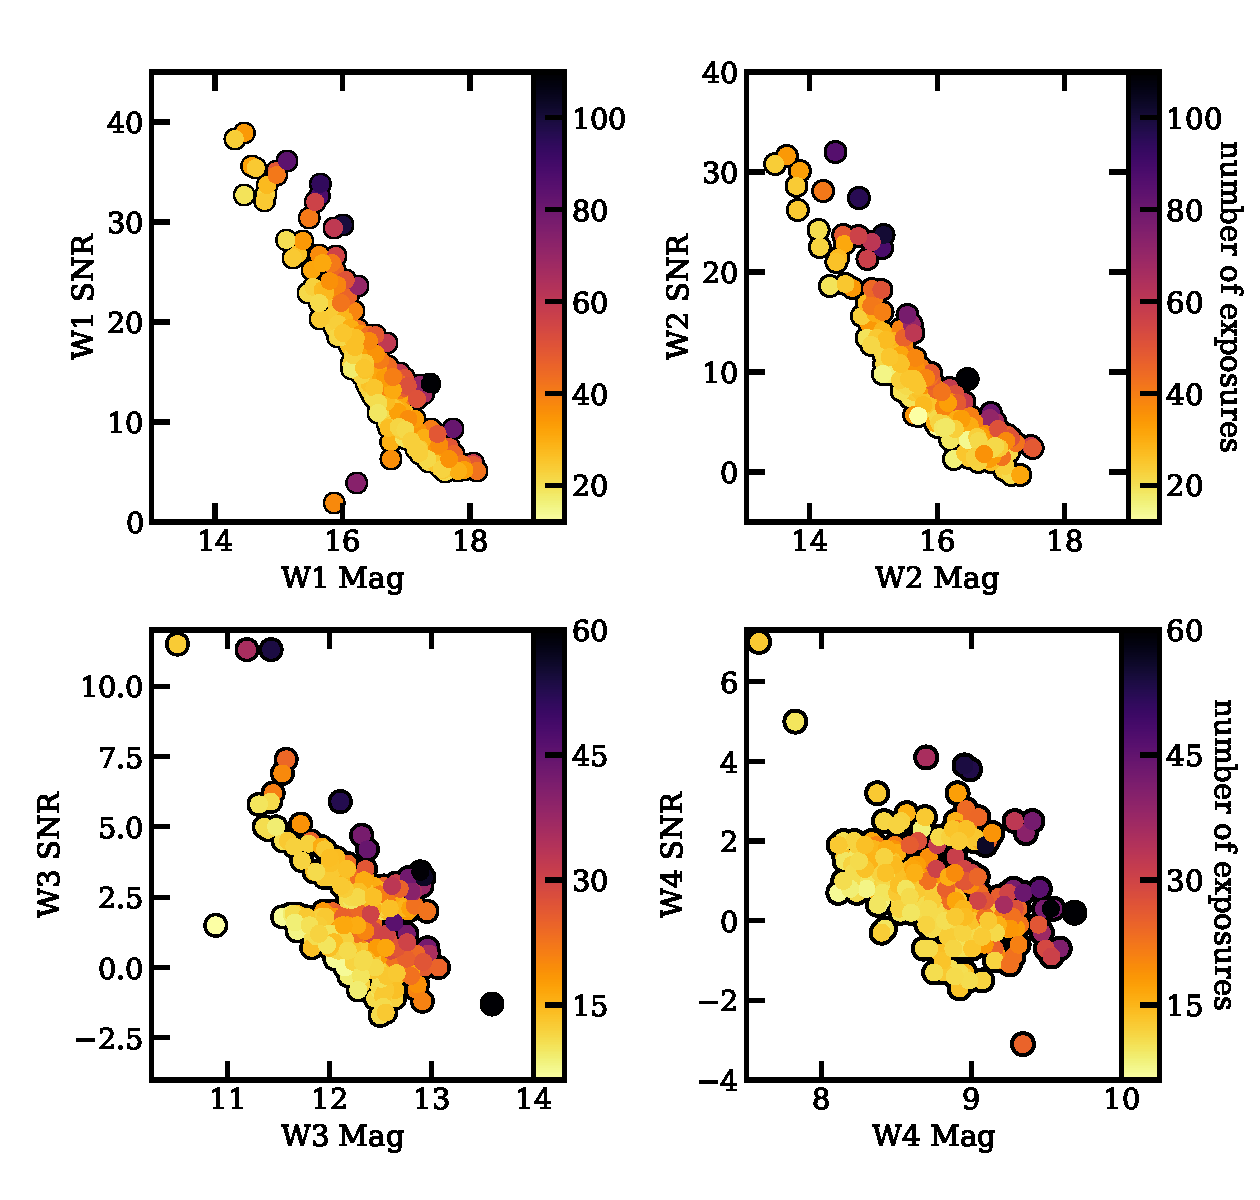
\includegraphics[width=8.6cm, clip,trim=6mm 6mm 0mm 6mm]
      {/cos_pc19a_npr/programs/quasars/highest_z/detections/WISEmag_vs_coverage_2x2_v1.pdf}
      \centering
      \vspace{-14pt}
      \caption[]{WISE W1/2/3/4 magnitude against signal-to-noise, 
        colour coded by w$x$cov the mean coverage depth, in each corresponding band.
      }
      \label{fig:WISEmag_vs_coverage}
    \end{figure}
    
    Table~\ref{tab:mir_detection} gives the detection rates for the
    VH$z$Qs in the MIR WISE W1-4 bands. 
    \begin{table}
      \begin{tabular}{l r l}
        \hline  \hline
        Selection   & number detected (\%) \\
        \hline  
        W1 SNR $> 2.0$                                             &  275  (64.9) \\
        W2 SNR $> 2.0$                                            &   255 (60.1) \\
        W1 $\land$ W2 SNR $> 2.0$                         &  \\
        W3 SNR $> 2.0$                                            &  99    (23.3) \\
        W4 SNR $> 2.0$                                            &  29    (6.8) \\
        Any W1/2/3/4 SNR $>2.0$                           & \\
        W1/2 SNR $< 2.0$ $\land$ W3 SNR $>2.0$ & \\
        \hline  \hline
      \end{tabular}
      \caption{}
      \label{tab:mir_detection}
    \end{table}

    \begin{table}
      \begin{tabular}{l r l}
        \hline  \hline
         \multirow{2}{*}{Selection}   & number detected \\ 
                                                   & (\% of full specrta) \\
        \hline  
        From ``Source'', ``Rejects'',                    & 245, 40  (67.2) \\
        W1 SNR $> 2.0$                                       &  279  (65.8) \\
        W2 SNR $> 2.0$                                       &  258 (60.8) \\
        W1 $\land$ W2 SNR $> 2.0$                    & 253   (59.7)  \\
        W3 SNR $> 2.0$                                     &  97    (22.9) \\
        W4 SNR $> 2.0$                                     &  33    (7.8) \\
%        Any W1/2/3/4 SNR $>2.0$                            & \\
        W1/2 SNR $< 2.0$ $\land$ W3 SNR $>2.0$ &  3 (0.7)\\
        \hline  \hline
      \end{tabular}
      \caption{Data from the AllWISE Source Catalog and AllWISE Reject Table, from the 
\href{https://irsa.ipac.caltech.edu/cgi-bin/Gator/nph-scan?submit=Select&projshort=WISE} {{\tt NASA/IPAC  Infrared Science Archive}}}
      \label{tab:mir_detection}
    \end{table}
    
    \begin{figure}
      %% trim=l b r t
      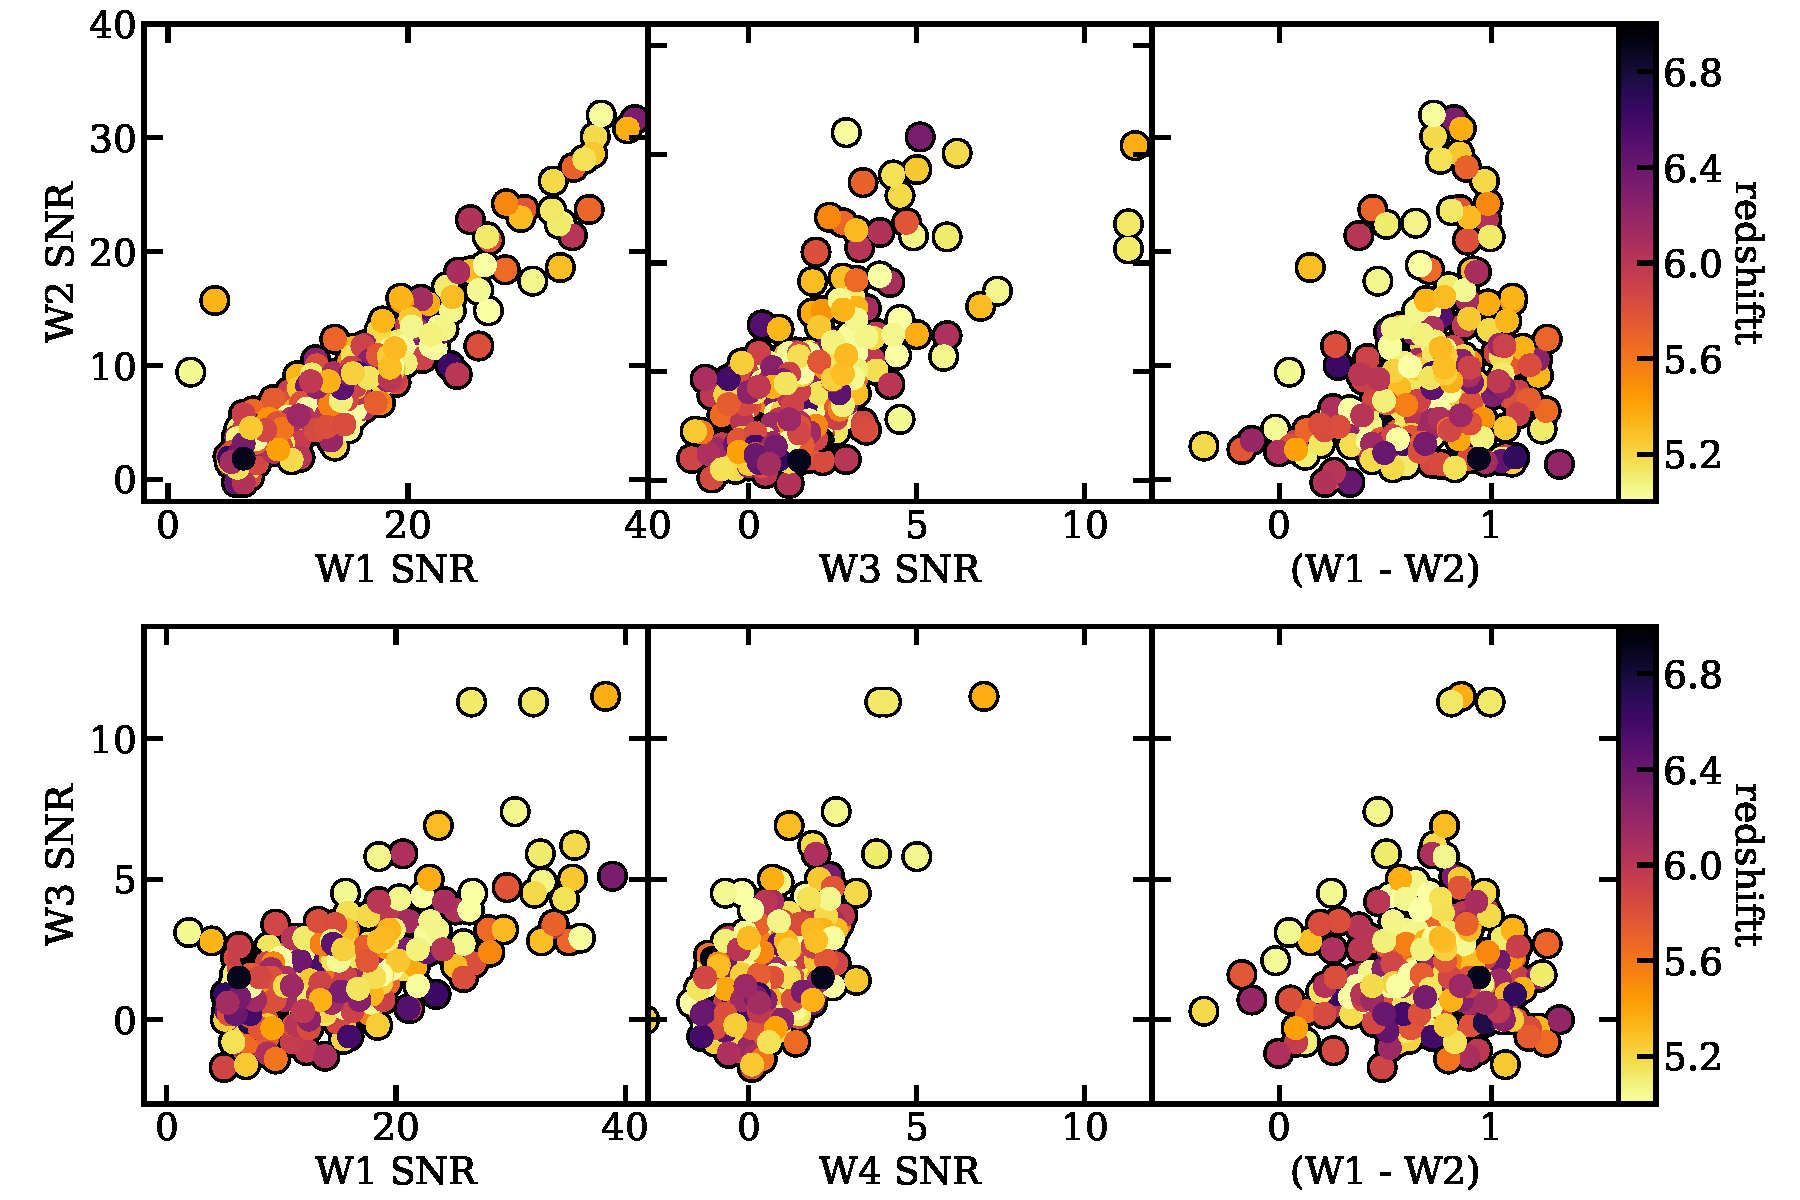
\includegraphics[width=8.6cm, clip,trim=2mm 0mm 2mm 0mm]
      {/cos_pc19a_npr/programs/quasars/highest_z/detections/WISEsnrW1W2W3W4_2by3_v1.pdf}
      \centering
      \vspace{-14pt}
      \caption[]{WISE signal-to-noise measures for the four bands, as well
        as for (W1-W2) colour.  The points are colour coded by redshift.}
      \label{fig:WISEmag_vs_coverage}
    \end{figure}

    \citet{Blain2013} 

    Recently, \citet{Assef2018} released two large catalogues of AGN 
    candidates identified across 30,000 deg$^2$ of extragalactic sky 
    from the WISE AllWISE Data Release. The ``R90'' catalogue, is 
    contains 4.5M AGN candidates at 90\% reliability (and $\approx$150 
    AGN candidates per deg$^2$) while the ``C75'' catalog 
    consists of 20.9M AGN candidates at 75\% completeness (and 
    ($\approx$700 AGN candidates per deg$^2$).  Crossmatching 
    out catalogue of 463 VH$z$Qs with these catalogues, produces 
    42 matches with	the R90 sample and 98 matches with the C75 sample. 
    Both catalogues unsurprisingly match to the ultraluminous quasar 
    SDSS J0100+2802 \citep{Wu2015} while the C75, but not the R90 catalogue 
    mathes to ULAS J1120+0641 \citep{Mortlock2011}. Neither catalogue 
    matches J1342+0928 \citep{Banados2018}. 

    %\subsubsection{
    Very High-$z$ Quasars Detected in WISE W3 and W4.


    \begin{figure}
      \centering
      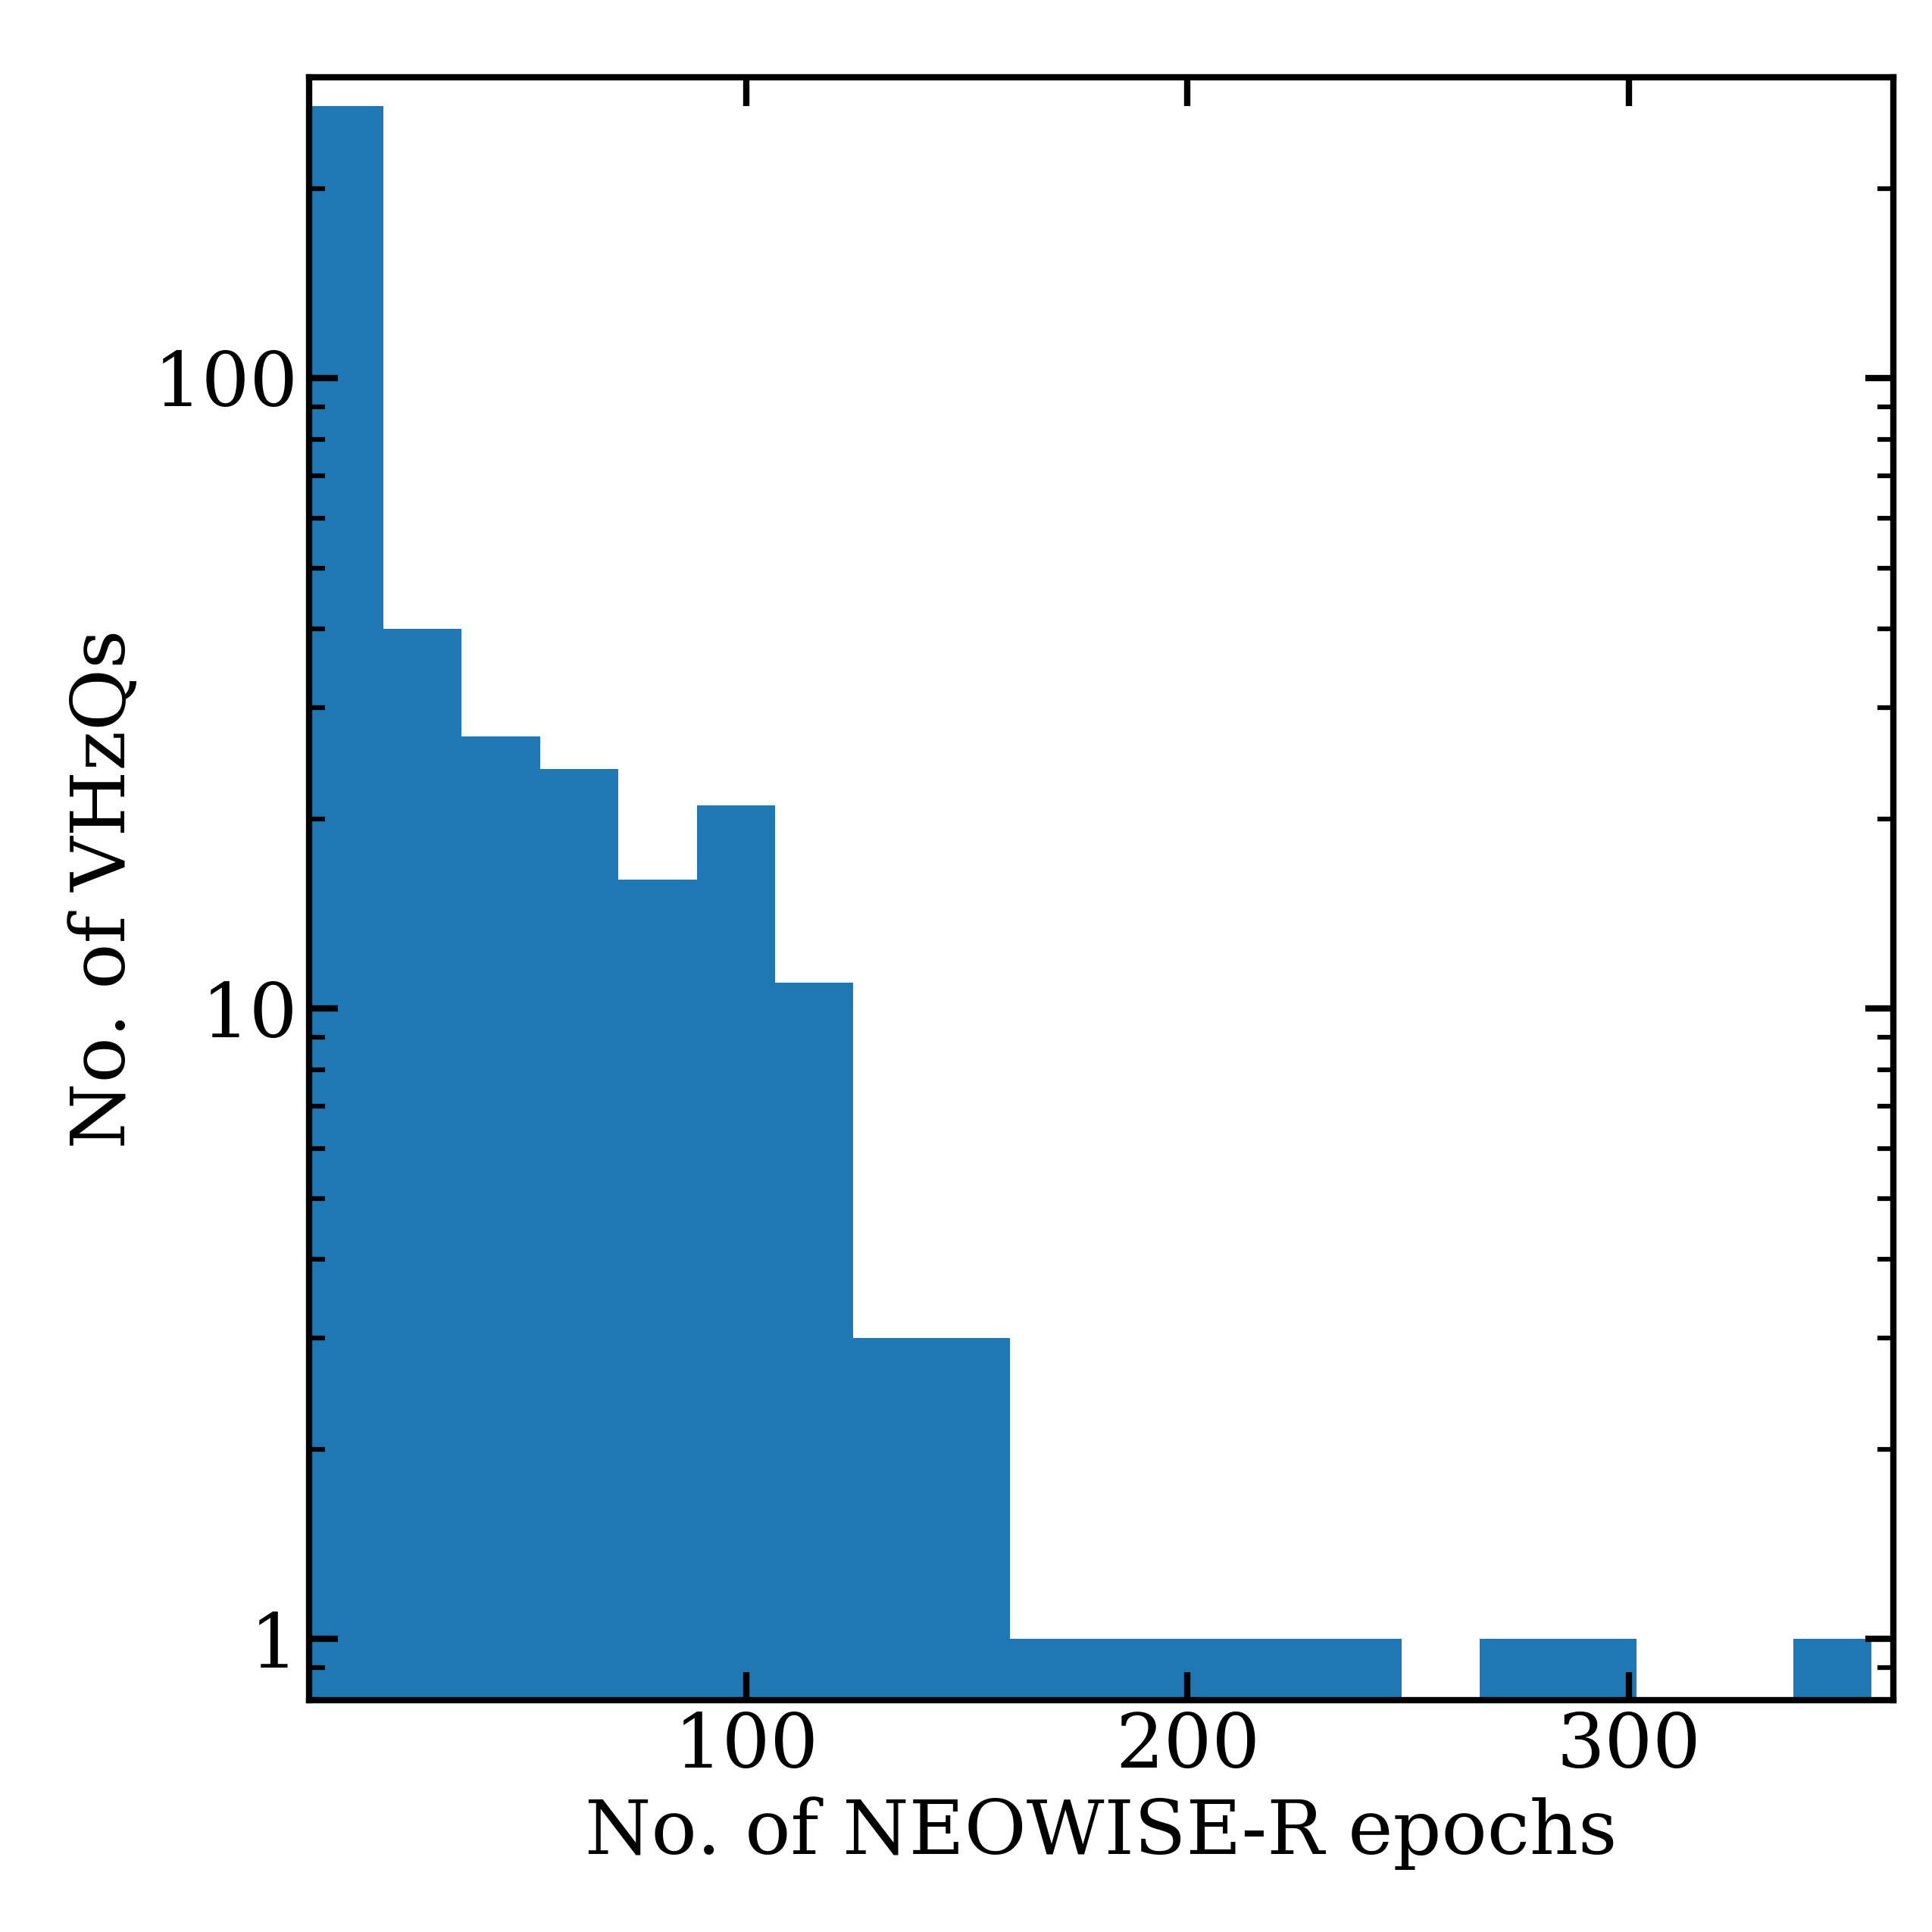
\includegraphics[width=8.5cm]
      {/cos_pc19a_npr/programs/quasars/highest_z/light_curves/MIR_LCs/NEOWISER_LC_histogramlog_20180827.png}
      \vspace{-16pt}
      \caption[]
      {Histogram showing the number of NEOWISE-R epochs and detections there are for each 
        VH$z$Q.} 
      \label{fig:MIR_LC_epochs}
    \end{figure}
    
\subsection{Variability}
VH$z$Qs, if accreting at, or above the Eddington Limit, might well have have large values of changing mass accretion rate, $\ddot{m_{\rm accr}}$. A consequence of this would be that these quasar exhibit signs of variability, most likely showing up in their UV/optical rest-frame spectra. We look for evidence of this variability signature in the NIR and MIR light-curves of the VH$z$Qs. As a guide, \civ enters the $Y$-band at redshift $z$=5.32 and exits at $z$=5.99, and enters the $J$-band at redshift $z=6.55$ and exits at $z$=7.57. \mgii enters the $H$-band at redshift $z=4.33$ and exits at $z=5.37$ and enters the $K$-band at redshift $z=6.25$ and exits at $7.50$.

Using the extended datasets described in Section~\ref{sec:NIR_data} and~\ref{sec:NIR_SQL}, we 

\begin{figure}
  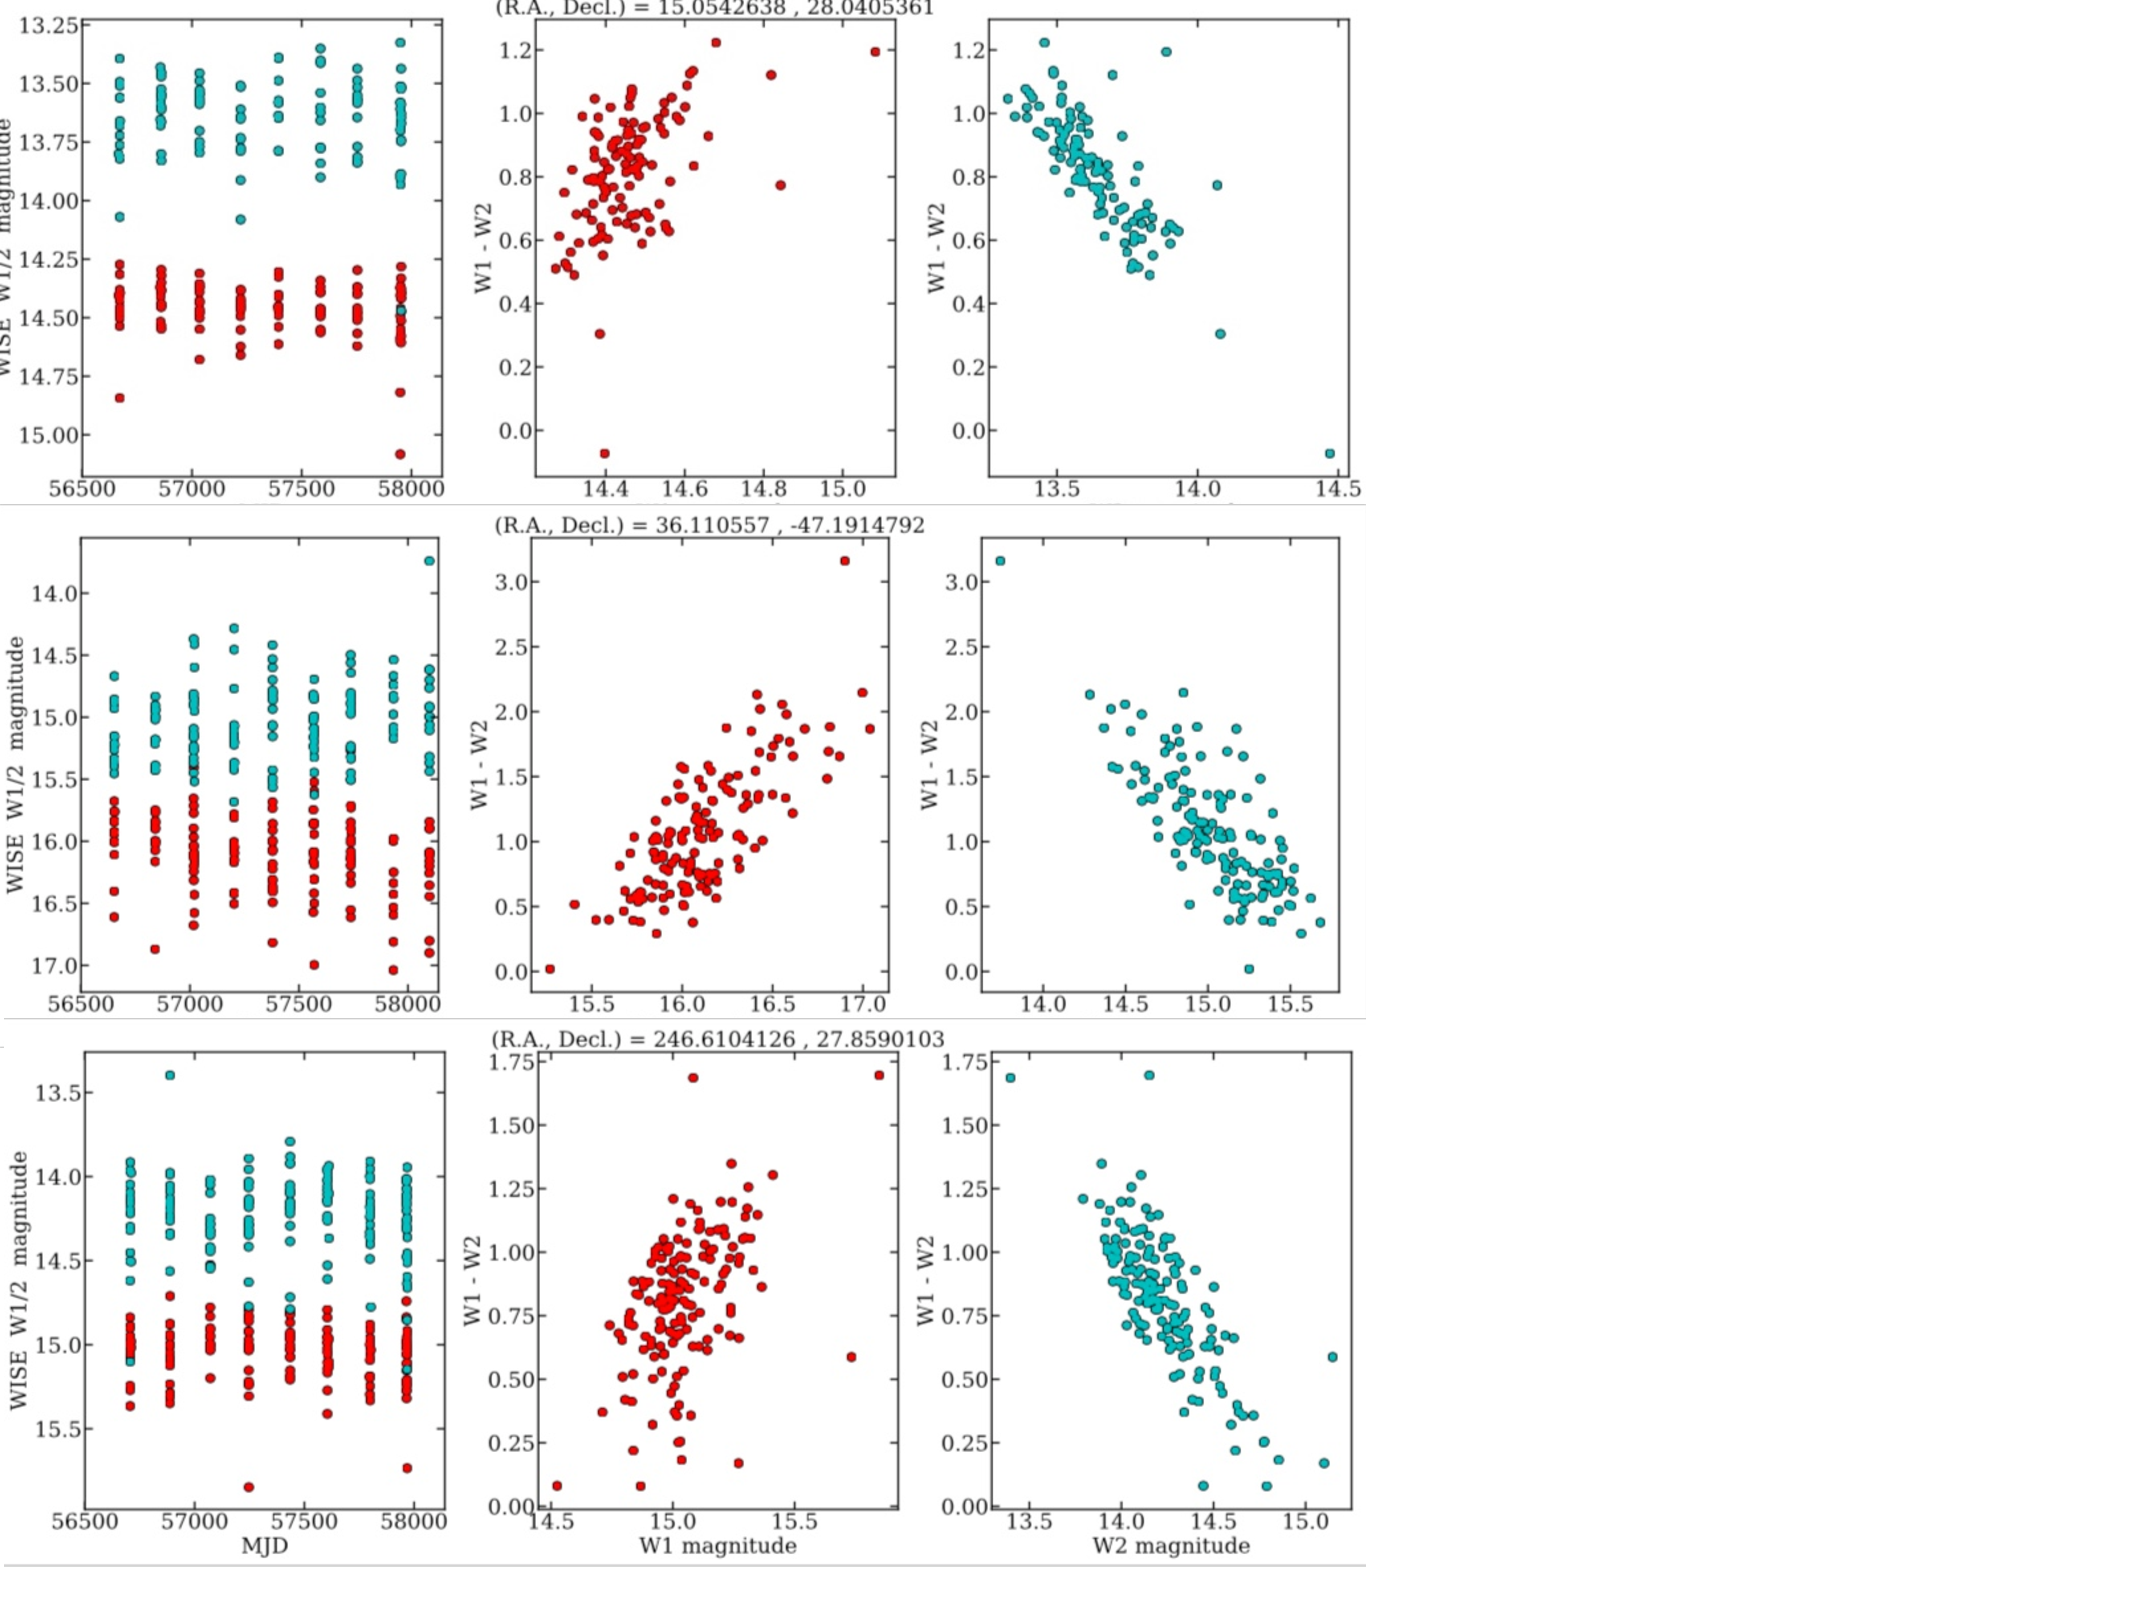
\includegraphics[width=8.5cm]
  {/cos_pc19a_npr/programs/quasars/highest_z/light_curves/MIR_LCs/three_MIR_LC_egs_20180827.pdf}
  \centering
  \caption[]
  {Here we show the MIR NEOWISE-R for J0100+2802 \citep{Wu2015}, J0224-4711 and  J1626+2751. 
    Red points are the W1 band; cyan points the W2 band.} 
  \label{fig::MIR_LC_3egs}
\end{figure}

Figure~\ref{fig:MIR_LC_epochs} gives the number of NEOWISE-R epochs and detections there are for each VH$z$Q, while 
Figure~\ref{fig:MIR_LC_3egs} presents three examples of the MIR lightcurves and
associated colour changes. Here we show J0100+2802 \citep{Wu2015}, J0224-4711 and  J1626+2751. 
{\bf NJC: What about NIR light-curves / combined light-curves}


%% On May 13, 2019, at 5:25 PM, Nicholas Cross <njc@roe.ac.uk> wrote:

%% I have also checked for QSOs with large differences in magnitude. At first I found loads of objects which appeared to have either the WFCAM or VISTA measurement more than 1 mag different from the mean. In fact initially there were 100 QSO/filter combinations. However, in many cases the average flux was less 0, or very close to zero, so I selected only objects where the average was >0. and >5 average flux error. This removed 80-90\%. I then found that many of the others had one of WFCAM or VISTA where the error bars were very large, so I removed ones where deltaMag<2.*deltaMagErr in either. This left me with 1 object or 2 if I reduced the change to 0.2 mag different from the mean:

The two with large differences are:

SDSSJ0349+0034, in K/Ks band: VSA = 18.36$\pm$0.10, WSA = 19.13$\pm$-0.24 and 

SDSSJ2220-0101, in J band: VSA = 19.38+/-0.04, WSA = 22.23+/-0.15


\subsection{Colours}
Currently, very high-redshift quasars are identified by their morphology, flux and colours in optical and infrared imaging data \citet{Fan1999, Mortlock2012} Quasars are generally selected to be point sources, but  be outliers from the stellar locus in colour space. For VH$z$Qs, the main technique is to look for objects with extreme optical-to-near-infrared colours The lack of proper motion can also help identified quasars \citep[e.g.][]{Lang2009}. 

\begin{figure*}
   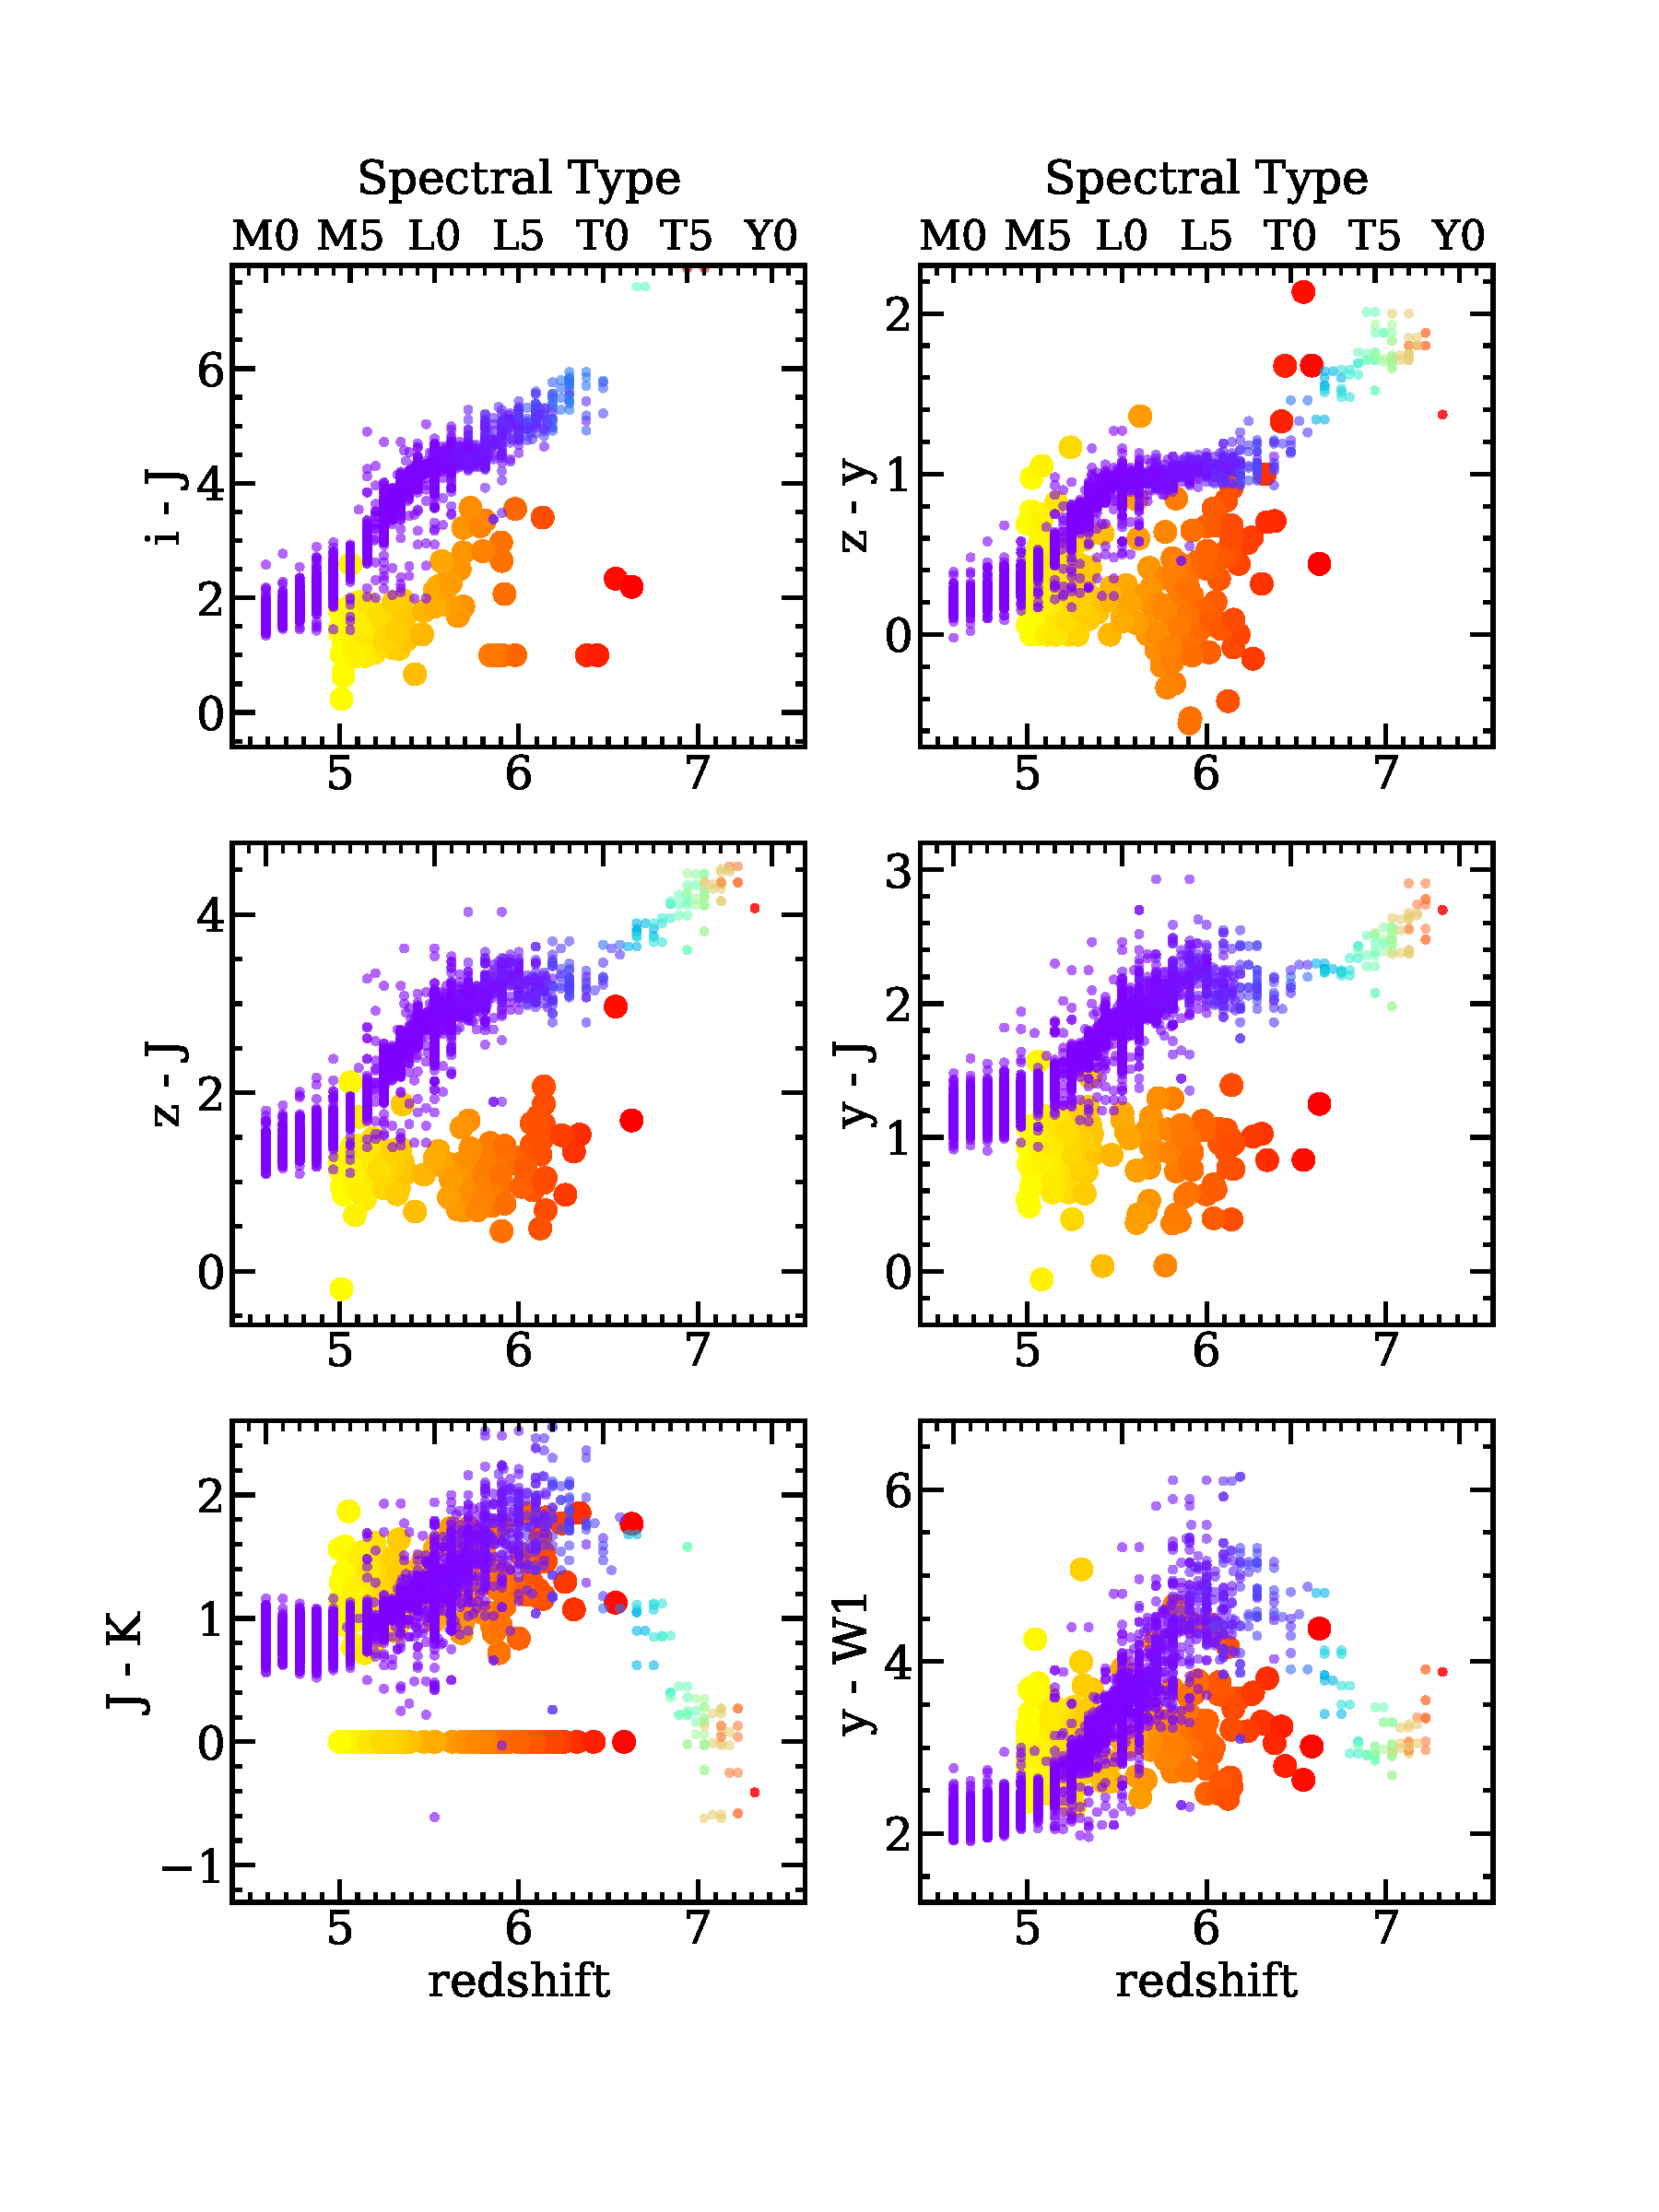
\includegraphics[width=18.0cm]
   {/cos_pc19a_npr/programs/quasars/highest_z/color_redshift/SpecType_vs_NIRcolors_20180704.pdf}
  \centering
   \caption[]
   {Infrared colour-spectral type and redshift plots for Late Type M/L/T dwarfs and the VH$z$Qs.
     {\it NB} I'm really not sure how Best et al. actually get their stellar sequence so clean. 
There are two types of spectral classification,  but restricting it to just SpT\_optn  or SpT\_nir removes
the blue or red end respectively. Hmmm....}
   \label{fig:SpecType_vs_NIRcolors}
 \end{figure*}

\begin{figure*}
   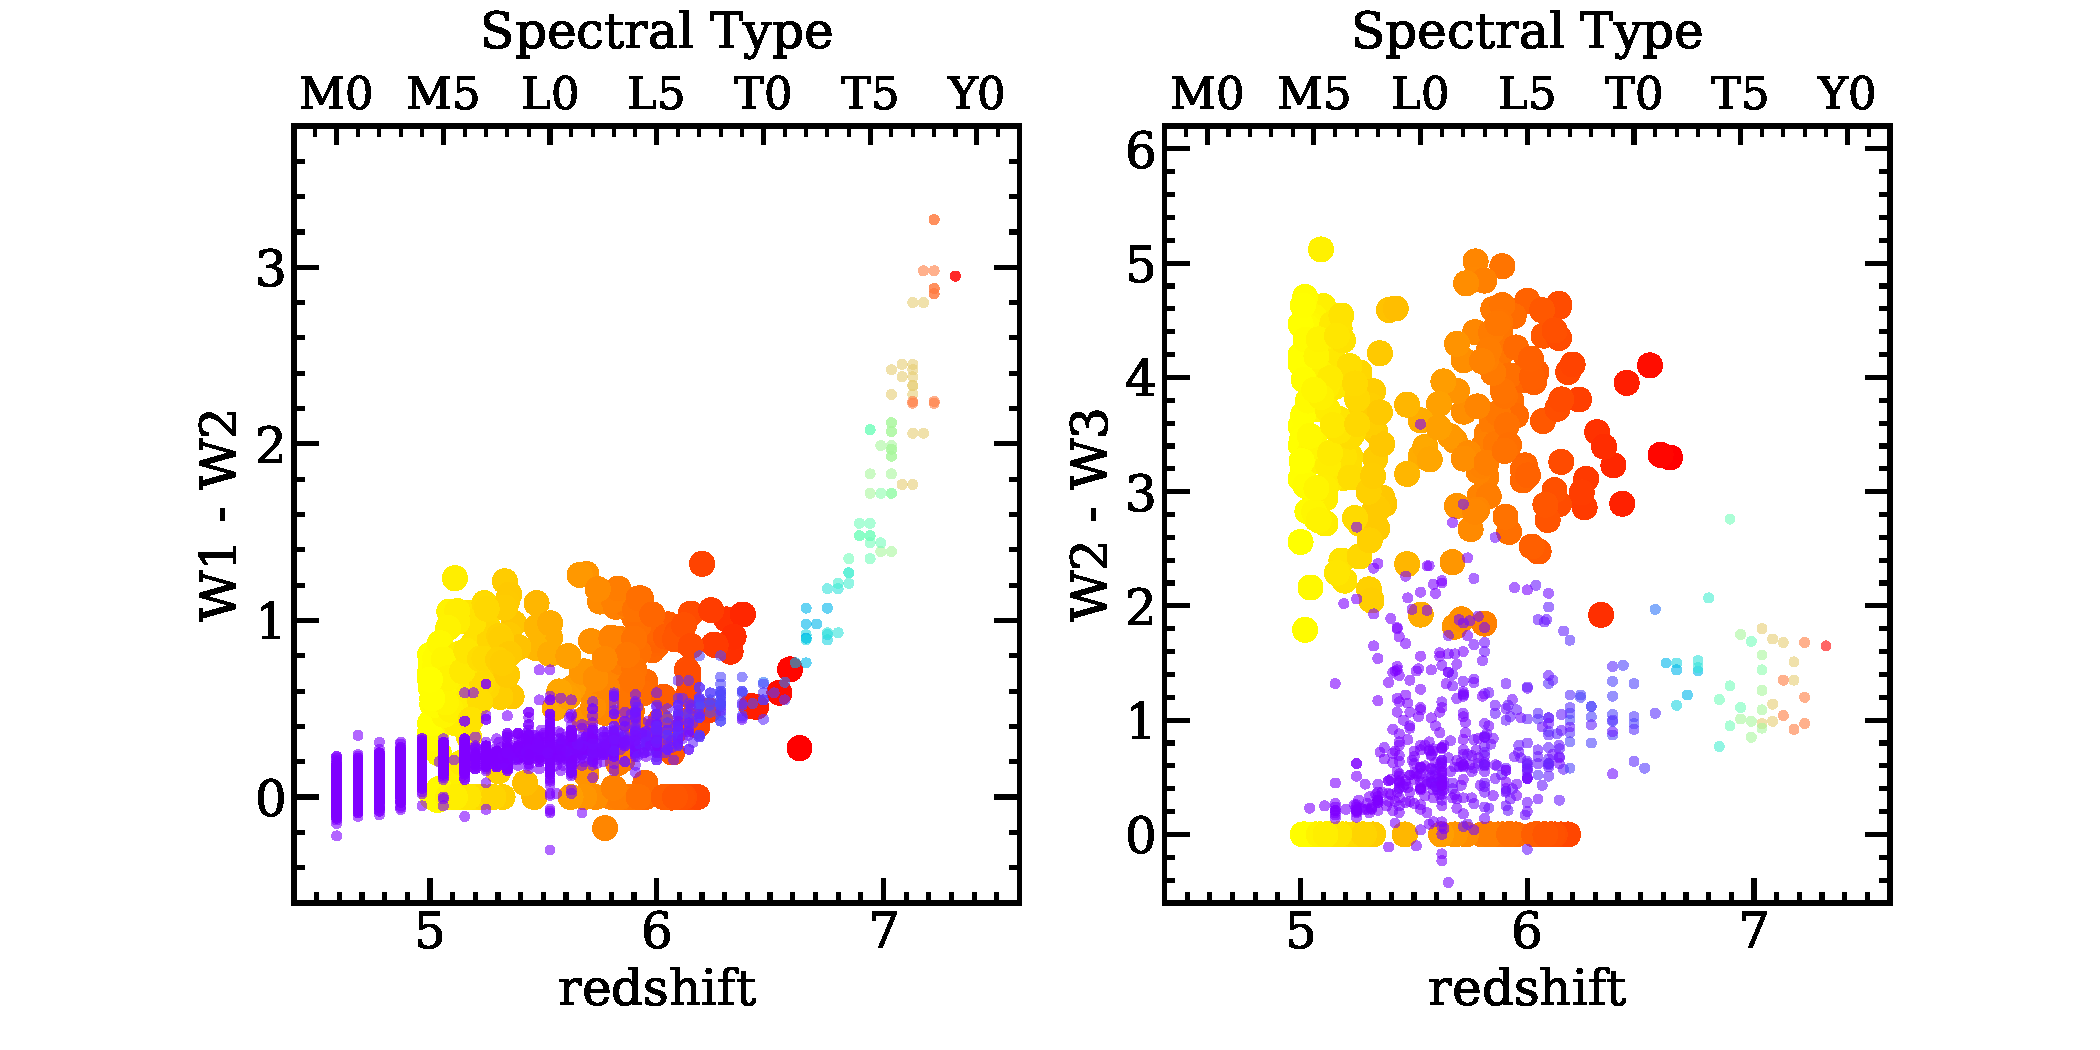
\includegraphics[width=18.0cm]
   {/cos_pc19a_npr/programs/quasars/highest_z/color_redshift/SpecType_vs_W1W2_W2W3colors_20180407.pdf}
  \centering
   \caption[]
   {Infrared colour-spectral type and redshift plots for Late Type M/L/T dwarfs and the VH$z$Qs.
}
   \label{fig:SpecType_vs_W1W2_W2W3colors}
 \end{figure*}


\subsection{L-$z$ Plane}
Having obtained an as-near-to-homogenous set of photometry as we can, 
we are now in a position to calculate the Absolute Magnitudes of the VH$z$Q 
sample and in particulare the absolute magnitude at rest-frame 1450\AA\ , $M_{1450}$, 
which is a key physical quantity and goes directly towards the quasar luminosity 
function and thus the reionization of hydrogen calculation. 

We calculate the Distance Modulus in the normal fashion, 
\begin{equation}
m_{1450} - M_{1450} = 5 \log \left (    \frac{ D_{\rm L}(z)}{\rm Mpc}  \right )  + 25 + K_{\rm corr}(X,z)
\end{equation}
where $m_{1450}$ is the apparent magnitude at 1450\AA\ ,  
%$M_{1450}$ is the absolute magnitude at 1450 \AA\ , 
$D_{\rm L}(z)$ is the luminosity distance and 
$K_{\rm corr}(X,z)$ is the $K$-correction which corrects for the effects of redshifting of the bandpass and the spectrum. 

The $m_{1450}$ apparent magnitude is derived from the $z-$, $y/Y-$ or $J-$band photometery.

The Pan-STARSS1 $z_{\rm PS1}$ and $y_{\rm PS1}$-bands approximatley
sample the redshift ranges $4.53\leq z \leq 5.45$ and $5.28\leq z \leq 6.47$, respectively 
for 1450\AA'\ emission, while the VIRCAM $Y_{\rm VIRCAM}-$ and $J_{\rm VIRCAM}$-bands 
cover $5.50\leq z \leq 6.57$ and $7.06\leq z \leq 8.16$. 

\citet{Ross2013} has a detailed discussion of the $K$-correction (see that papers' Appendix B). 
The key result in that paper is, if quasars are described as having a power-law slope, 
$\alpha^{\nu}$ in spectral flux density, i.e., $f_\nu(\nu) \propto \nu^{\alpha_{\nu}}$ (as is conventional) 
then 
\begin{equation}
K_{\rm corr}(z) = -2.5 (1 + \alpha_{\nu}) \log[1 + z].
\end{equation}
Here the $[-2.5 \log(1 + z)]$ term corrects for the effective narrowing of the filter width with redshift, (the ``bandpass correction'') and the $[-2.5 \alpha^{\nu} \log(1 + z)]$ term takes into account the spectral index correction. The bandpass correction is approximately $\approx -1.945$ at redshift $z=5$ decreasing to $-2.32$ at redshift $z=7.50$. 


%At $z=5.00$, the rest-frame 1450\AA\ emission is redshifted to 8700\AA\ observed, i.e., in the $z$-band, while at $z=6.00$, $z=5.00$


\begin{figure*}
  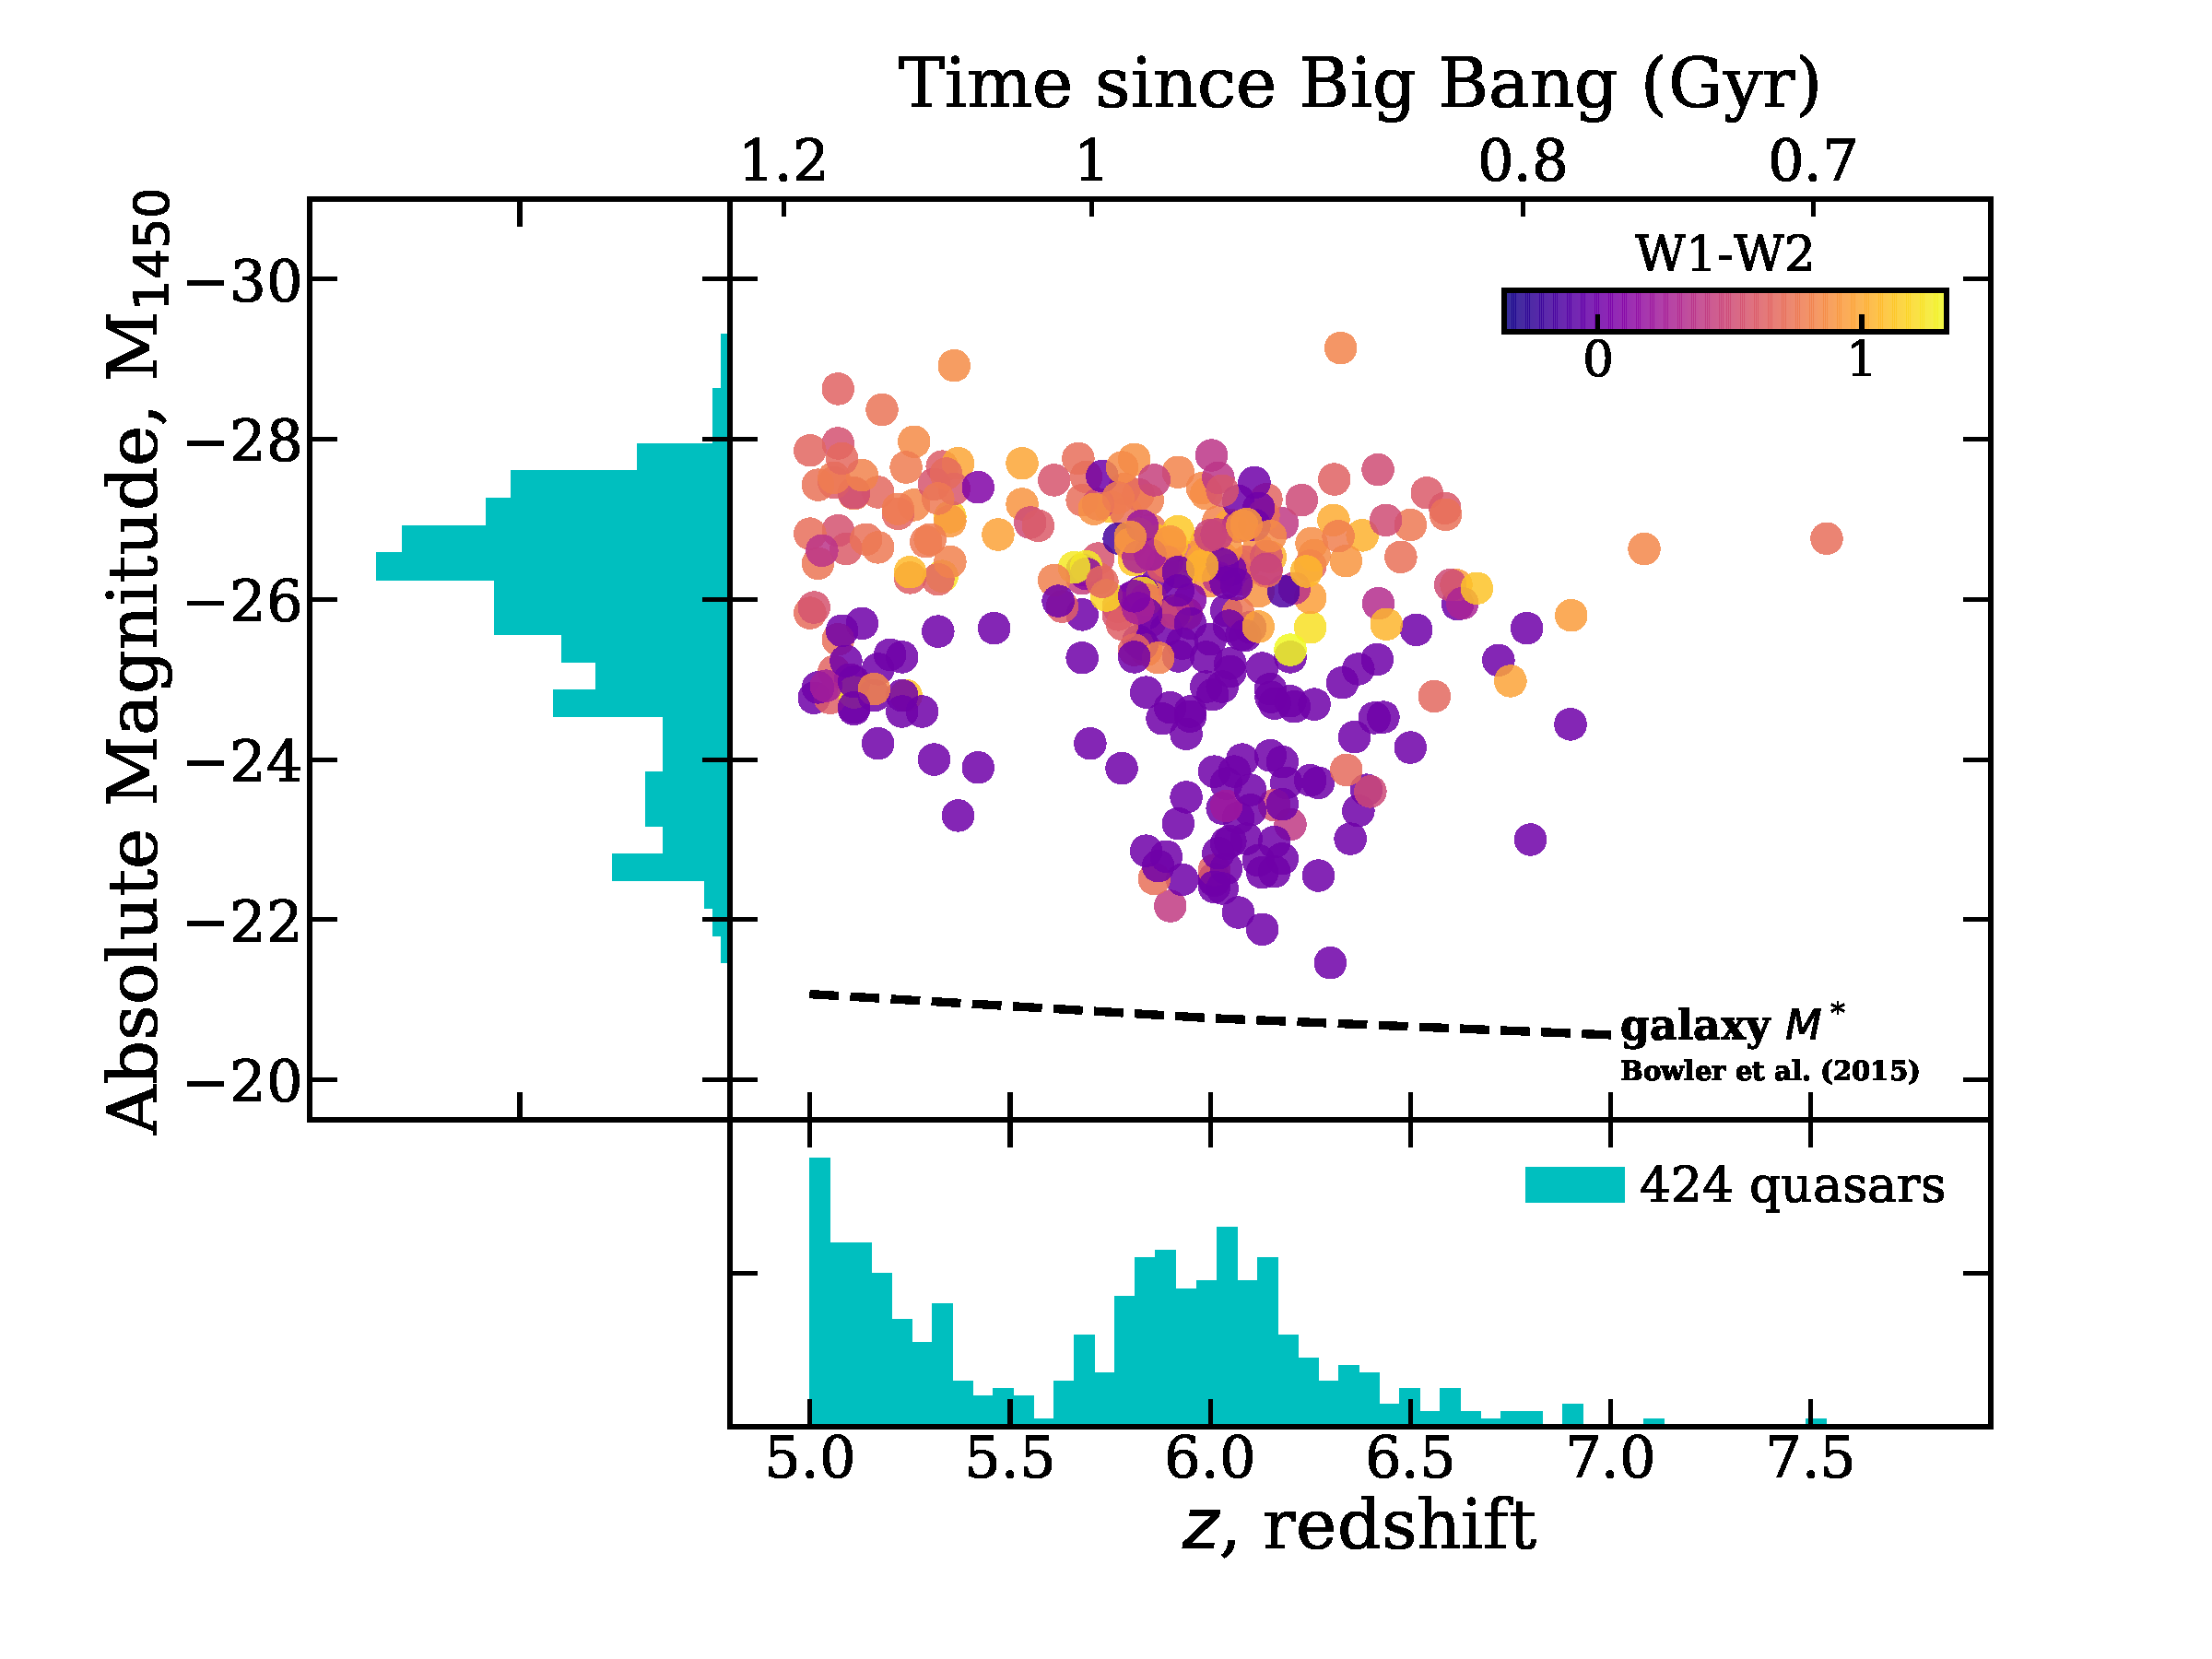
\includegraphics[width=18.0cm]
  {/cos_pc19a_npr/programs/quasars/highest_z/Lz/VHzQ_Lz_20180702.pdf}
  \centering
  \caption[]
  {The spectral bands used by different survey telescopes and that are relevant here.}
  \label{fig:Lz}
\end{figure*}


%%%%%%%%%%%%%%%%%%%%%%%%%%%%%%%%%%%%%%%%%%%%%%%%%%%%%%%%%%%%%%%%%%
%%%%%%%%%%%%%%%%%%%%%%%%%%%%%%%%%%%%%%%%%%%%%%%%%%%%%%%%%%%%%%%%%%
%%
%%  S E C T I O  N   7         S E C T I O  N   7           S E C T I O  N   7       S E C T I O  N   7
%%  S E C T I O  N   7         S E C T I O  N   7           S E C T I O  N   7       S E C T I O  N   7
%%  S E C T I O  N   7         S E C T I O  N   7           S E C T I O  N   7       S E C T I O  N   7
%%
%%%%%%%%%%%%%%%%%%%%%%%%%%%%%%%%%%%%%%%%%%%%%%%%%%%%%%%%%%%%%%%%%%
%%%%%%%%%%%%%%%%%%%%%%%%%%%%%%%%%%%%%%%%%%%%%%%%%%%%%%%%%%%%%%%%%%
\section{Discussion and Conclusions}
\label{sec:conclusions}
In this study, we have, for the first time, ompiled the list of all
$z>5$ spectroscopically confirmed quasars. We have assemble the NIR
($y/Y, J, H, K/K_{s}$) and MIR (WISE W1/2/3/4) photometry for these
objects, given their detection rates and SEDs. We find that: 

%%
We can gain a good appreciation for what these missions will discover
by collating the datasets we currently have. 

\begin{itemize}
    \item Lorem ipsum dolor sit amet, consectetur adipiscing
      elit. Aliquam porta sodales est, vel cursus risus porta non. Vivamus
      vel pretium velit. Sed fringilla suscipit felis, nec iaculis lacus
      convallis ac. 
    \item Fusce pellentesque condimentum dolor, quis vehicula
      tortor hendrerit sed. Class aptent taciti sociosqu ad litora torquent
      per conubia nostra, per inceptos himenaeos. Etiam interdum tristique
      diam eu blandit. Donec in lacinia libero.
    \item Sed elit massa, eleifend non sodales a, commodo ut felis. Sed id
      pretium felis. Vestibulum et turpis vitae quam aliquam convallis. Sed
      id ligula eu nulla ultrices tempus. Phasellus mattis erat quis metus
      dignissim malesuada. Nulla tincidunt quam volutpat nibh facilisis
      euismod. Cras vel auctor neque. Nam quis diam risus.
\end{itemize}
Nunc lacus nibh, convallis ac lobortis ut, tempus ac lectus. Maecenas
eu elit massa. Nulla vel lacus lorem. Proin et lobortis
tortor. Phasellus ultrices nisl non enim porttitor dictum. Curabitur
nec nunc ac nibh ornare elementum. Nunc ultrices hendrerit
ultricies. Aliquam dapibus semper est et gravida. Etiam cursus, massa
eget tempor elementum, lectus urna feugiat nisi, eget sagittis.

\subsection*{Author Contributions}   
N.P.R. initiated the project, compiled the list of $z>5.00$ quasars, wrote most of the analysis code, developed the the plotting scripts, and developed and wrote the initial and subsequent drafts of the manuscript.
%%
N.J.G.C. supplied the critical near-infrared expertise and database for which the bulk of the project relies. N.J.G.C. also contributed directly to the writing of the manuscript.
%%



\subsection*{Availability of Data and computer analysis codes} 
All materials, databases, data tables and code are fully available at: 
\href{https://github.com/d80b2t/VHzQ}{\tt https://github.com/d80b2t/VHzQ}


\section*{Acknowledgements}
NPR acknowledges support from the STFC and the Ernest Rutherford Fellowship scheme. 

We thank Mike Read at the ROE WFAU for help with the WFCAM Science Archiv (WSA), and 
also the VISTA Science Archive (VSA). We thank Bernie Shiao at STScI for help with the Pan-STARRS1 DR1 CasJobs interface. 

This paper heavily used \href{http://www.star.bris.ac.uk/~mbt/topcat/}{TOPCAT} (v4.4)
\citep[][]{Taylor2005, Taylor2011}.
%%
This research made use of \href{http://www.astropy.org}{\tt Astropy}, 
a community-developed core Python package for Astronomy 
\citep{AstropyCollaboration2013, AstropyCollaboration2018}. 

The Pan-STARRS1 Surveys (PS1) and the PS1 public science archive have
been made possible through contributions by the Institute for
Astronomy, the University of Hawaii, the Pan-STARRS Project Office,
the Max-Planck Society and its participating institutes, the Max
Planck Institute for Astronomy, Heidelberg and the Max Planck
Institute for Extraterrestrial Physics, Garching, The Johns Hopkins
University, Durham University, the University of Edinburgh, the
Queen's University Belfast, the Harvard-Smithsonian Center for
Astrophysics, the Las Cumbres Observatory Global Telescope Network
Incorporated, the National Central University of Taiwan, the Space
Telescope Science Institute, the National Aeronautics and Space
Administration under Grant No. NNX08AR22G issued through the Planetary
Science Division of the NASA Science Mission Directorate, the National
Science Foundation Grant No. AST-1238877, the University of Maryland,
Eotvos Lorand University (ELTE), the Los Alamos National Laboratory,
and the Gordon and Betty Moore Foundation.

This project used data obtained with the Dark Energy Camera (DECam)
and the NOAO Data Lab, The Data Lab is operated by the National
Optical Astronomy Observatory, the national center for ground-based
nighttime astronomy in the United States operated by the Association
of Universities for Research in Astronomy (AURA) under cooperative
agreement with the National Science Foundation.

This publication makes use of data products from the Wide-field
Infrared Survey Explorer, which is a joint project of the University
of California, Los Angeles, and the Jet Propulsion
Laboratory/California Institute of Technology, and NEOWISE, which is a
project of the Jet Propulsion Laboratory/California Institute of
Technology. WISE and NEOWISE are funded by the National Aeronautics
and Space Administration.

CasJobs was originally developed by the Johns Hopkins University/
Sloan Digital Sky Survey (JHU/SDSS) team. With their permission, MAST
used version 3.5.16 to construct CasJobs-based tools for GALEX,
Kepler, the Hubble Source Catalog, and PanSTARRS.

This research has made use of the SVO Filter Profile Service
(http://svo2.cab.inta-csic.es/theory/fps/) supported from the Spanish
MINECO through grant AyA2014-55216 
%%
The SVO Filter Profile Service\footnote{Rodrigo, C., Solano, E., Bayo, A. http://ivoa.net/documents/Notes/SVOFPS/index.html}
describes the Spanish VO Filter Profile Service. 
The Filter Profile Service Access Protocol. Rodrigo, C., Solano, E. http://ivoa.net/documents/Notes/SVOFPSDAL/index.html

\newpage





\appendix
%\section{Filter Curves}\label{sec:filters} 
%From the SVO Filter Profile Service\footnote{http://svo2.cab.inta-csic.es/svo/theory/fps/}.

\section{A. Photometric Bands and Conversions}\label{sec:filters} 
    Due to the differing normalizations between the
    SDSS and  UKIDSS photometric systems, certain corrections are required.  To present
    our data in the  purest sense, all the NIR magnitudes from UKIDSS
    (originally AB magnitudes)  were corrected to Vega magnitudes as
    suggested in \citet{Hewett2006}.
    
    Although ULAS magnitudes are reported in terms of Vega and SDSS
    magnitudes are reported in AB terms for the most part whenever an
    optical-NIR color was calculated both magnitudes were left in their
    default term.
    
\begin{table*}
  \begin{center}
   \caption{Adapted from Table 9 of \citet{Peth2011}. 
CTIO/DECam, PanSTARRS/PS1, LSST
%References: www.cfht.hawaii.edu/Instruments/Filters/wircam.html
Filter only values. 
All wavelengths in ${\buildrel _{\circ} \over {\mathrm{A}}}$. 
%%
%%
From \citet{GonzalezFernandez2018} 
$Z_{\rm AB}   -  Z_{\rm Vega}  = 0.502$;  
$Y_{\rm AB}  -  Y_{\rm Vega}    = 0.600 $;
$J_{\rm AB}   -  J_{\rm Vega}    = 0.916  $;
$H_{\rm AB}  -  H_{\rm Vega}    = 1.366 $;
$Ks_{\rm AB}  -  Ks_{\rm Vega}  = 1.827 $;
%%
and the CASU Vega to AB conversions v1.3:: 
	Z,Y,J,H,Ks were: 0.524, 0.618, 0.937, 1.384, 1.839. 
%%
So, $\Delta$(vs. Gonzalez-Fernandez)::
	(11.2,     1.1,    5.4,     1.6,    0.1) millimags. 
$\Delta$(vsCASU v1.3)::
	(-10.8, -16.9, -15.6,  -16.4, -11.9) millimags. 
}
    \setlength{\tabcolsep}{4pt}
     \begin{tabular}{l r r r  c l l}
      %% https://www.gemini.edu/sciops/instruments/magnitudes-and-fluxes
      %% http://wise2.ipac.caltech.edu/docs/release/allsky/expsup/sec4_4h.html#conv2ab
       %%
       %% http://svo2.cab.inta-csic.es/svo/theory/fps/index.php?mode=browse&gname=UKIRT&gname2=WFCAM
      %%                                                                                     
     %% emails around 16 Aug 2018, Carlos Rodrigo
      %% 
     %%     (-2.5)*(log10( ZP_in_Jy / 3631.0)) 
      \hline
      \hline
      Band & $\lambda_{\rm eff}  $ 
              &  $\lambda_{\rm min} $ 
              & $\lambda_{\rm max} $ 
              & W$_{\rm eff}$
              & \multicolumn{2}{c}{AB - Vega  Transformations} \\
      \hline
      % {\it u} & 3551  &  3005 &  4000 &  581 & $u$ = $u_{AB}$ - 0.927 \\
      % {\it u_{\rm LSST}} &	3733 &	3182 &	4082 &	?? \\
       $g_{\rm HSC}$    &  	4633   &     3940     &   5546	&  1460       &    $g_{\rm HSC}$         &$  = g_{\rm AB} + 0.097 $ \\
      $g_{\rm LSST}$      &     4730     &	  3877    &	   5665   &  1333   &  $g_{\rm LSST}$       &$ = g_{\rm AB} +  0.083 $ \\   %% from SVO 3921.4 
      $g_{\rm DECam}$  &      4734     &   3939    &    5528   &   1133        &  $g_{\rm DECam} $    &$  = g_{\rm AB} + 0.083 $ \\	     
       $g_{\rm PS1}$        &    4776    &    3943    &    5593   &   1167        &  $g_{\rm PS1}$         &$  = g_{\rm AB} + 0.080 $ \\   %% from SVO; e.g.   (-2.5)*(log10(3909.1/3631.0)) 
      &&&&&&\\
      $r_{\rm HSC}$         &    6104     &   5325    &   7071	&   1503       & $r_{\rm HSC}   $       &$     = r_{\rm AB} - 0.151 $ \\
      $r_{\rm PS1}$         &    6130    & 	  5386    &    7036   &   1318       &  $r_{\rm PS1}   $       &$     = r_{\rm AB} - 0.153 $ \\ %% from SVO; e.g.   (-2.5)*(log10(3151.4/3631.0)) 
      $r_{\rm LSST}$       &     6139    &	  5375    &    7055   &   1338      &  $r_{\rm LSST}   $       &$    = r_{\rm AB} - 0.155 $ \\	
      $r_{\rm DECam}$   &      6345    &    5506    &    7238   &   1379      &  $r_{\rm DECam}$       &$   = r_{\rm AB} - 0.192 $ \\	     
      &&&&&&\\
      $i_{\rm PS1}$         &    7485    &     6778    &    8304   &   1243      &  $i_{\rm PS1}    $       &$   = i_{\rm AB} - 0.369 $ \\  %% 2584.6
      $i_{\rm LSST}$       &     7487    &	  6765    &     8325   &   1209      &  $i_{\rm LSST}   $       &$    = i_{\rm AB} - 0.369 $ \\   %% 2583.9
      $i_{\rm HSC}$         &   7633    &     6791    &     8658	&   1483       &  $i_{\rm PS1}    $       &$   = i_{\rm AB} - 0.396 $ \\  %% 2521.6
      $i_{\rm DECam}$   &      7750   &	  6950    &     8646    &   1371      &  $i_{\rm DECam} $     &$  = i_{\rm AB} - 0.415 $        \\	   
      &&&&&&\\
      $z_{\rm PS1}$        &    8658    &	 8028    &      9346   &      966      &  $z_{\rm PS1}   $      &$    = z_{\rm AB} - 0.508 $       \\
      $z_{\rm LSST}$      &     8669   & 	 8035    &      9375   &      994     &   $z_{\rm LSST}  $      &$    = z_{\rm AB} - 0.509 $     \\
      $Z_{\rm VIRCAM}$  &     8762   & 	 8157    &      9400   &      978    &   $Z_{\rm VIRCAM}  $   &$    = Z_{\rm AB} - 0.513 $     \\
      $Z_{\rm WFCAM}$  &     8802   & 	 8129    &      9457   &      926    &   $Z_{\rm WFCAM}  $   &$    = Z_{\rm AB} - 0.514 $     \\
      $z_{\rm HSC}$        &    8915  &   	8280     &      9498	&    793      & 	$Z_{\rm HSC} $         &$    = Z_{\rm AB} - 0.512$     \\
      $z_{\rm DECam}$  &      9216   & 	 8360    &    10166   &   1502      &  $z_{\rm DECam} $     &$   = z_{\rm AB} - 0.521 $ \\
      &&&&&&\\
      $y_{\rm PS1}$       &       9603    &  9100    &    10838  &     615       &  $y_{\rm PS1}    $       &$   = y_{\rm AB} -  0.541 $ \\
      $y_{\rm LSST}$      &       9677   &	 9089    &    10859  &     810         &  $y_{\rm LSST}  $      &$    = y_{\rm AB} - 0.546 $ \\
      $Y_{\rm DECam}$   &      9876   &	  9355    &      10730   &    676      &  $Y_{\rm DECam}  $   &$  =Y_{\rm AB} - 0.570 $ \\
      $Y_{\rm HSC}$       &      9976   &    9000    & 	10931  &   1386    &  $Y_{\rm HSC}  $   &$  =Y_{\rm AB} - 0.580 $ \\
      $Y_{\rm WFCAM}$    &   10305    &   9790      &   10810   &   1020     & $Y_{\rm WFCAM}$     &$ =  Y_{AB}  - 0.617$           \\
      $Y_{\rm VIRCAM}$     &    10184    &   9427      &   10977   &    905        & $Y_{\rm VIRCAM} $     &$ = Y_{AB}  - 0.601 $          \\
      &&&&&&\\
      $J_{\rm 2MASS}$       &   12350   &       10806  & 	14068  &  1624       &  $J_{\rm 2MASS}  $     & $= J_{AB}    - 0.894  $         \\
      $J_{\rm VIRCAM} $     &   12464   &      11427   &    13759   &  1628     &  $J_{\rm VIRCAM}  $     & $= J_{AB}    - 0.921  $         \\
      $J_{\rm WFCAM} $    &    12483   &     11690  &    13280   &   1590      & $J_{\rm WFCAM}$     & $= J_{AB}    - 0.919 $          \\
      &&&&&&\\
      $W_{\rm Wircam}$   &    14514    &    13890   &    15166   &   1020    & $W_{\rm Wircam} $    & $= W_{AB}  -  1.163$           \\
      &&&&&&\\
      $H_{\rm WFCAM}$    &    16313     &    14920  &    17840   &   2920    & $H_{\rm WFCAM} $   & $= H_{AB}  - 1.379$          \\
      $H_{\rm VIRCAM}$      &    16310    &    14604   &    18422   &   2833     & $H_{\rm VIRCAM}$      & $= H_{AB}  - 1.368 $        \\
      $H_{\rm 2MASS}$      & 16620        & 	14787  &   18231   & 2509      & $H_{\rm 2MASS}$      & $= H_{AB}  - 1.374 $        \\
      &&&&&&\\
      $K$s$_{\rm VIRCAM}$     &    21337    &    19333  &    23674   &   3055     & $K$s$_{\rm VIRCAM}$      & $ = K$s$_{AB} - 1.83  $          \\ 
      $K$s$_{\rm 2MASS}$     &   21590    & 	19544  &   23552        &   2619      & $K$s$_{\rm 2MASS}$      & $ = K$s$_{AB} -  1.84  $          \\ 
      $K_{\rm WFCAM}$     &    22010     &    20290 &    23800         &   3510          & $K_{\rm WFCAM}$     & $ = K_{AB} - 1.90  $          \\ 
      &&&&&&\\
      WISE W1               &    33526    &    27541  &    38724   &    6626    & W1                        &   = W1$_{\rm AB} - 2.699$ \\
      WISE W2               &    46028    &    39633  &    53414   &  10423    & W2                        &   = W2$_{\rm AB} - 3.339$ \\
      WISE W3               &  115608    &    74430  &  172613   &  55056    & W3                        &   = W3$_{\rm AB} - 5.174$ \\
      WISE W4               &  228172    &  195201  &  279107   &  41017    & W4                        &   = W4$_{\rm AB} - 6.66$ \\
      \hline
      \hline
      \label{tab:filter_details}
    \end{tabular}
     \end{center}
\end{table*}
https://www.gemini.edu/sciops/instruments/magnitudes-and-fluxes


\section{Near-Infrared WFCAM Science Archive SQL queries}\label{sec:SQL}
Here we give the receipe and SQL that returned the near-infrared photometry 
for the VH$z$Qs from the  WFCAM Science Archive. 

The data are on the WFCAM Science Archive: \href{wsa.roe.ac.uk}{\tt wsa.roe.ac.uk}. 
Access the User Login form \href{WFCAM Science Archive}{\tt wsa.roe.ac.uk/login.html} 
with these credentials::
\begin{itemize}
    \item Username: {\tt WSERV1000} 
    \item password: {\tt highzqso} 
    \item community: {\tt nonsurvey}
\end{itemize}
Then going to the
\href{http://wsa.roe.ac.uk:8080/wsa/SQL_form.jsp}{{\tt Free Form SQL
Query}} page the Database release {\tt WSERV1000v20180716} can be
accessed which contains all the data we use here.

We {\it nota bene} a few things. First, the quantity {\tt aperJky3}
and {\tt aperJky3Err} are found in the {\tt wserv1000MapRemeasAver}
and {\tt wserv1000MapRemeasurement}, so care has to be taken to return
unique column names (otherwise e.g.
\href{http://docs.astropy.org/en/stable/io/fits/}{astropy.io.fits}
will crash).  As such, we alias {\tt aver.aperJky3} to {\tt
aperJky3Aver} and likewise for the error quantity. Aliases will be
necessary in some cases anyway, because some queries can be done
sensibly on multiple instances of the same table. Other times, one may
join tables on quantities such as {\tt catalogueID} or {\tt
apertureID}, where you are meaning the same thing, but aliases would
again be sensible.

Second, the {\tt RA} and {\tt DEC} values returned by the WSA are in radians, if
used directly. To return values in degrees, use a selection with an alias, e.g. 
{\tt RA as RADeg} and {\tt DEC as DECDeg}.

\onecolumn
\lstset{upquote=true}

\noindent
{\bf The following SQL will return 
the best magnitude in each band for each QSO.}


\begin{lstlisting}[
           language=SQL,
           showspaces=false,
           basicstyle=\ttfamily,
           numbers=left,
           numberstyle=\tiny,
           commentstyle=\color{gray}
        ]
SELECT 
qso.qsoName,  qso.ra as raJ2000, qso.dec as decJ2000, 
aver.apertureID,  aver.aperJky3 as aperJky3Aver, 
aver.aperJky3Err as aperJky3AverErr, aver.sumWeight, 
aver.ppErrBits as ppErrBitsAver, m.mjdObs, 
m.filterID, remeas.aperJky3, 
remeas.aperJky3Err, 
w.weight, remeas.ppErrBits, 
m.project

FROM 
finalQsoCatalogue as qso,  
MapApertureIDshighzQsoMap as ma,  
wserv1000MapRemeasAver as aver,  
wserv1000MapRemeasurement as remeas,  
MapProvenance as v,  
wserv1000MapAverageWeights as w, 
MapFrameStatus as mfs, 
Multiframe as m  

WHERE 
qso.qsoID=ma.objectID and 
ma.apertureID=aver.apertureID and 
aver.apertureID=remeas.apertureID and 
aver.catalogueID=v.combicatID and 
v.avSetupID=1 and 
v.catalogueID=remeas.catalogueID and 
w.combicatID=v.combicatID and 
w.catalogueID=v.catalogueID and 
w.apertureID=aver.apertureID and 
mfs.catalogueID=remeas.catalogueID and 
m.multiframeID=mfs.multiframeID and 
mfs.programmeID=10999 and 
mfs.mapID=1 
order by v.combicatID, m.mjdObs
\end{lstlisting}

\twocolumn


\section{Near-Infrared VISTA Science Archive SQL queries}\label{sec:SQL}
In a very similar manner to the WSA, we give here the details on how to access
the VISTA Science Archive (VSA)

At the \href{http://horus.roe.ac.uk/vsa/login.html}{VSA Login}, enter 
with these credentials::
\begin{itemize}
    \item Username: {\tt VSERV1000} 
    \item password: {\tt highzqso} 
    \item community: {\tt proprietary}
\end{itemize}
Then head to the \href{http://horus.roe.ac.uk:8080/vdfs/VSQL_form.jsp}{Freeform SQL Query} page where the database release to use is {\tt VSERV1000v20180716}. 

\onecolumn
\lstset{upquote=true}

\noindent
Then the following SQL will return the values in
Table~\ref{tab:THE_TABLE}.

\begin{lstlisting}[
           language=SQL,
           showspaces=false,
           basicstyle=\ttfamily,
           numbers=left,
           numberstyle=\tiny,
           commentstyle=\color{gray}
        ]
SELECT 
qso.qsoName,  qso.ra as raJ2000, qso.dec as decJ2000, 
aver.apertureID,  aver.aperJky3 as aperJky3Aver, 
aver.aperJky3Err as aperJky3AverErr, aver.sumWeight, 
aver.ppErrBits as ppErrBitsAver, m.mjdObs, 
m.filterID, remeas.aperJky3, 
remeas.aperJky3Err, 
w.weight, remeas.ppErrBits, 
m.project

FROM 
finalQsoCatalogue as qso,  
MapApertureIDshighzQsoMap as ma,  
vserv1000MapRemeasAver as aver,  
vserv1000MapRemeasurement as remeas,  
MapProvenance as v,  
vserv1000MapAverageWeights as w, 
MapFrameStatus as mfs, 
Multiframe as m  

WHERE 
qso.qsoID=ma.objectID and 
ma.apertureID=aver.apertureID and 
aver.apertureID=remeas.apertureID and 
aver.catalogueID=v.combicatID and 
v.avSetupID=1 and 
v.catalogueID=remeas.catalogueID and 
w.combicatID=v.combicatID and 
w.catalogueID=v.catalogueID and 
w.apertureID=aver.apertureID and 
mfs.catalogueID=remeas.catalogueID and 
m.multiframeID=mfs.multiframeID and 
mfs.programmeID=10999 and 
mfs.mapID=1 
order by v.combicatID, m.mjdObs
\end{lstlisting}

\twocolumn









%%%%%%%%%%%%%%%%%%%%%%%%%%%%%%%%%%%%%%%%%%%%%%%%%%%%%%%%%%%%%%%%%%%%
%%%%%%%%%%%%%%%%%%%%%%%%%%%%%%%%%%%%%%%%%%%%%%%%%%%%%%%%%%%%%%%%%%%%

%\bibliographystyle{apj}
\bibliographystyle{mn2e}
\bibliography{tester_mnras}

\end{document}
